
%% bare_jrnl_compsoc.tex
%% V1.3
%% 2007/01/11
%% by Michael Shell
%% See:
%% http://www.michaelshell.org/
%% for current contact information.
%%
%% This is a skeleton file demonstrating the use of IEEEtran.cls
%% (requires IEEEtran.cls version 1.7 or later) with an IEEE Computer
%% Society journal paper.
%%
%% Support sites:
%% http://www.michaelshell.org/tex/ieeetran/
%% http://www.ctan.org/tex-archive/macros/latex/contrib/IEEEtran/
%% and
%% http://www.ieee.org/

%%*************************************************************************
%% Legal Notice:
%% This code is offered as-is without any warranty either expressed or
%% implied; without even the implied warranty of MERCHANTABILITY or
%% FITNESS FOR A PARTICULAR PURPOSE! 
%% User assumes all risk.
%% In no event shall IEEE or any contributor to this code be liable for
%% any damages or losses, including, but not limited to, incidental,
%% consequential, or any other damages, resulting from the use or misuse
%% of any information contained here.
%%
%% All comments are the opinions of their respective authors and are not
%% necessarily endorsed by the IEEE.
%%
%% This work is distributed under the LaTeX Project Public License (LPPL)
%% ( http://www.latex-project.org/ ) version 1.3, and may be freely used,
%% distributed and modified. A copy of the LPPL, version 1.3, is included
%% in the base LaTeX documentation of all distributions of LaTeX released
%% 2003/12/01 or later.
%% Retain all contribution notices and credits.
%% ** Modified files should be clearly indicated as such, including  **
%% ** renaming them and changing author support contact information. **
%%
%% File list of work: IEEEtran.cls, IEEEtran_HOWTO.pdf, bare_adv.tex,
%%                    bare_conf.tex, bare_jrnl.tex, bare_jrnl_compsoc.tex
%%*************************************************************************

% *** Authors should verify (and, if needed, correct) their LaTeX system  ***
% *** with the testflow diagnostic prior to trusting their LaTeX platform ***
% *** with production work. IEEE's font choices can trigger bugs that do  ***
% *** not appear when using other class files.                            ***
% The testflow support page is at:
% http://www.michaelshell.org/tex/testflow/




% Note that the a4paper option is mainly intended so that authors in
% countries using A4 can easily print to A4 and see how their papers will
% look in print - the typesetting of the document will not typically be
% affected with changes in paper size (but the bottom and side margins will).
% Use the testflow package mentioned above to verify correct handling of
% both paper sizes by the user's LaTeX system.
%
% Also note that the "draftcls" or "draftclsnofoot", not "draft", option
% should be used if it is desired that the figures are to be displayed in
% draft mode.
%
% The Computer Society usually requires 10pt for submissions.
%
\documentclass[10pt,journal,letterpaper,compsoc]{IEEEtran}
%
% If IEEEtran.cls has not been installed into the LaTeX system files,
% manually specify the path to it like:
% \documentclass[12pt,journal,compsoc]{../sty/IEEEtran}





% Some very useful LaTeX packages include:
% (uncomment the ones you want to load)


% *** MISC UTILITY PACKAGES ***
%
%\usepackage{ifpdf}
% Heiko Oberdiek's ifpdf.sty is very useful if you need conditional
% compilation based on whether the output is pdf or dvi.
% usage:
% \ifpdf
%   % pdf code
% \else
%   % dvi code
% \fi
% The latest version of ifpdf.sty can be obtained from:
% http://www.ctan.org/tex-archive/macros/latex/contrib/oberdiek/
% Also, note that IEEEtran.cls V1.7 and later provides a builtin
% \ifCLASSINFOpdf conditional that works the same way.
% When switching from latex to pdflatex and vice-versa, the compiler may
% have to be run twice to clear warning/error messages.


%%extra packages ------ 
\usepackage{longtable}   
\usepackage{float} %allows the use of [H] to force positioning of figures
\usepackage{subfigure}
\usepackage{hyperref} %used in references now  --- it shoud be removed
\usepackage{amssymb}
\usepackage[neveradjust]{paralist} %compact lists
\usepackage{amsthm}

\newtheorem*{theory}{Theory}

% *** CITATION PACKAGES ***
%
\ifCLASSOPTIONcompsoc
  % IEEE Computer Society needs nocompress option
  % requires cite.sty v4.0 or later (November 2003)
  % \usepackage[nocompress]{cite}
\else
  % normal IEEE
  % \usepackage{cite}
\fi
% cite.sty was written by Donald Arseneau
% V1.6 and later of IEEEtran pre-defines the format of the cite.sty package
% \cite{} output to follow that of IEEE. Loading the cite package will
% result in citation numbers being automatically sorted and properly
% "compressed/ranged". e.g., [1], [9], [2], [7], [5], [6] without using
% cite.sty will become [1], [2], [5]--[7], [9] using cite.sty. cite.sty's
% \cite will automatically add leading space, if needed. Use cite.sty's
% noadjust option (cite.sty V3.8 and later) if you want to turn this off.
% cite.sty is already installed on most LaTeX systems. Be sure and use
% version 4.0 (2003-05-27) and later if using hyperref.sty. cite.sty does
% not currently provide for hyperlinked citations.
% The latest version can be obtained at:
% http://www.ctan.org/tex-archive/macros/latex/contrib/cite/
% The documentation is contained in the cite.sty file itself.
%
% Note that some packages require special options to format as the Computer
% Society requires. In particular, Computer Society  papers do not use
% compressed citation ranges as is done in typical IEEE papers
% (e.g., [1]-[4]). Instead, they list every citation separately in order
% (e.g., [1], [2], [3], [4]). To get the latter we need to load the cite
% package with the nocompress option which is supported by cite.sty v4.0
% and later. Note also the use of a CLASSOPTION conditional provided by
% IEEEtran.cls V1.7 and later.





% *** GRAPHICS RELATED PACKAGES ***
%
%\ifCLASSINFOpdf
   \usepackage[pdftex]{graphicx}
  % declare the path(s) where your graphic files are
   \graphicspath{{figures}}
  % and their extensions so you won't have to specify these with
  % every instance of \includegraphics
  % \DeclareGraphicsExtensions{.pdf,.jpeg,.png}
%\else
  % or other class option (dvipsone, dvipdf, if not using dvips). graphicx
  % will default to the driver specified in the system graphics.cfg if no
  % driver is specified.
%   \usepackage[dvips]{graphicx}
  % declare the path(s) where your graphic files are
   %\graphicspath{{./figures/}}
  % and their extensions so you won't have to specify these with
  % every instance of \includegraphics
   %\DeclareGraphicsExtensions{.eps}
%\fi
% graphicx was written by David Carlisle and Sebastian Rahtz. It is
% required if you want graphics, photos, etc. graphicx.sty is already
% installed on most LaTeX systems. The latest version and documentation can
% be obtained at: 
% http://www.ctan.org/tex-archive/macros/latex/required/graphics/
% Another good source of documentation is "Using Imported Graphics in
% LaTeX2e" by Keith Reckdahl which can be found as epslatex.ps or
% epslatex.pdf at: http://www.ctan.org/tex-archive/info/
%
% latex, and pdflatex in dvi mode, support graphics in encapsulated
% postscript (.eps) format. pdflatex in pdf mode supports graphics
% in .pdf, .jpeg, .png and .mps (metapost) formats. Users should ensure
% that all non-photo figures use a vector format (.eps, .pdf, .mps) and
% not a bitmapped formats (.jpeg, .png). IEEE frowns on bitmapped formats
% which can result in "jaggedy"/blurry rendering of lines and letters as
% well as large increases in file sizes.
%
% You can find documentation about the pdfTeX application at:
% http://www.tug.org/applications/pdftex





% *** MATH PACKAGES ***
%
%\usepackage[cmex10]{amsmath}
% A popular package from the American Mathematical Society that provides
% many useful and powerful commands for dealing with mathematics. If using
% it, be sure to load this package with the cmex10 option to ensure that
% only type 1 fonts will utilized at all point sizes. Without this option,
% it is possible that some math symbols, particularly those within
% footnotes, will be rendered in bitmap form which will result in a
% document that can not be IEEE Xplore compliant!
%
% Also, note that the amsmath package sets \interdisplaylinepenalty to 10000
% thus preventing page breaks from occurring within multiline equations. Use:
%\interdisplaylinepenalty=2500
% after loading amsmath to restore such page breaks as IEEEtran.cls normally
% does. amsmath.sty is already installed on most LaTeX systems. The latest
% version and documentation can be obtained at:
% http://www.ctan.org/tex-archive/macros/latex/required/amslatex/math/





% *** SPECIALIZED LIST PACKAGES ***
%
%\usepackage{algorithmic}
% algorithmic.sty was written by Peter Williams and Rogerio Brito.
% This package provides an algorithmic environment fo describing algorithms.
% You can use the algorithmic environment in-text or within a figure
% environment to provide for a floating algorithm. Do NOT use the algorithm
% floating environment provided by algorithm.sty (by the same authors) or
% algorithm2e.sty (by Christophe Fiorio) as IEEE does not use dedicated
% algorithm float types and packages that provide these will not provide
% correct IEEE style captions. The latest version and documentation of
% algorithmic.sty can be obtained at:
% http://www.ctan.org/tex-archive/macros/latex/contrib/algorithms/
% There is also a support site at:
% http://algorithms.berlios.de/index.html
% Also of interest may be the (relatively newer and more customizable)
% algorithmicx.sty package by Szasz Janos:
% http://www.ctan.org/tex-archive/macros/latex/contrib/algorithmicx/




% *** ALIGNMENT PACKAGES ***
%
\usepackage{array}
% Frank Mittelbach's and David Carlisle's array.sty patches and improves
% the standard LaTeX2e array and tabular environments to provide better
% appearance and additional user controls. As the default LaTeX2e table
% generation code is lacking to the point of almost being broken with
% respect to the quality of the end results, all users are strongly
% advised to use an enhanced (at the very least that provided by array.sty)
% set of table tools. array.sty is already installed on most systems. The
% latest version and documentation can be obtained at:
% http://www.ctan.org/tex-archive/macros/latex/required/tools/


%\usepackage{mdwmath}
%\usepackage{mdwtab}
% Also highly recommended is Mark Wooding's extremely powerful MDW tools,
% especially mdwmath.sty and mdwtab.sty which are used to format equations
% and tables, respectively. The MDWtools set is already installed on most
% LaTeX systems. The lastest version and documentation is available at:
% http://www.ctan.org/tex-archive/macros/latex/contrib/mdwtools/


% IEEEtran contains the IEEEeqnarray family of commands that can be used to
% generate multiline equations as well as matrices, tables, etc., of high
% quality.


\usepackage{eqparbox}
% Also of notable interest is Scott Pakin's eqparbox package for creating
% (automatically sized) equal width boxes - aka "natural width parboxes".
% Available at:
% http://www.ctan.org/tex-archive/macros/latex/contrib/eqparbox/





% *** SUBFIGURE PACKAGES ***
%\ifCLASSOPTIONcompsoc
%\usepackage[tight,normalsize,sf,SF]{subfigure}
%\else
%\usepackage[tight,footnotesize]{subfigure}
%\fi
% subfigure.sty was written by Steven Douglas Cochran. This package makes it
% easy to put subfigures in your figures. e.g., "Figure 1a and 1b". For IEEE
% work, it is a good idea to load it with the tight package option to reduce
% the amount of white space around the subfigures. Computer Society papers
% use a larger font and \sffamily font for their captions, hence the
% additional options needed under compsoc mode. subfigure.sty is already
% installed on most LaTeX systems. The latest version and documentation can
% be obtained at:
% http://www.ctan.org/tex-archive/obsolete/macros/latex/contrib/subfigure/
% subfigure.sty has been superceeded by subfig.sty.


%\ifCLASSOPTIONcompsoc
%  \usepackage[caption=false]{caption}
%  \usepackage[font=normalsize,labelfont=sf,textfont=sf]{subfig}
%\else
%  \usepackage[caption=false]{caption}
%  \usepackage[font=footnotesize]{subfig}
%\fi
% subfig.sty, also written by Steven Douglas Cochran, is the modern
% replacement for subfigure.sty. However, subfig.sty requires and
% automatically loads Axel Sommerfeldt's caption.sty which will override
% IEEEtran.cls handling of captions and this will result in nonIEEE style
% figure/table captions. To prevent this problem, be sure and preload
% caption.sty with its "caption=false" package option. This is will preserve
% IEEEtran.cls handing of captions. Version 1.3 (2005/06/28) and later 
% (recommended due to many improvements over 1.2) of subfig.sty supports
% the caption=false option directly:
%\ifCLASSOPTIONcompsoc
%  \usepackage[caption=false,font=normalsize,labelfont=sf,textfont=sf]{subfig}
%\else
%  \usepackage[caption=false,font=footnotesize]{subfig}
%\fi
%
% The latest version and documentation can be obtained at:
% http://www.ctan.org/tex-archive/macros/latex/contrib/subfig/
% The latest version and documentation of caption.sty can be obtained at:
% http://www.ctan.org/tex-archive/macros/latex/contrib/caption/




% *** FLOAT PACKAGES ***
%
%\usepackage{fixltx2e}
% fixltx2e, the successor to the earlier fix2col.sty, was written by
% Frank Mittelbach and David Carlisle. This package corrects a few problems
% in the LaTeX2e kernel, the most notable of which is that in current
% LaTeX2e releases, the ordering of single and double column floats is not
% guaranteed to be preserved. Thus, an unpatched LaTeX2e can allow a
% single column figure to be placed prior to an earlier double column
% figure. The latest version and documentation can be found at:
% http://www.ctan.org/tex-archive/macros/latex/base/



%\usepackage{stfloats}
% stfloats.sty was written by Sigitas Tolusis. This package gives LaTeX2e
% the ability to do double column floats at the bottom of the page as well
% as the top. (e.g., "\begin{figure*}[!b]" is not normally possible in
% LaTeX2e). It also provides a command:
%\fnbelowfloat
% to enable the placement of footnotes below bottom floats (the standard
% LaTeX2e kernel puts them above bottom floats). This is an invasive package
% which rewrites many portions of the LaTeX2e float routines. It may not work
% with other packages that modify the LaTeX2e float routines. The latest
% version and documentation can be obtained at:
% http://www.ctan.org/tex-archive/macros/latex/contrib/sttools/
% Documentation is contained in the stfloats.sty comments as well as in the
% presfull.pdf file. Do not use the stfloats baselinefloat ability as IEEE
% does not allow \baselineskip to stretch. Authors submitting work to the
% IEEE should note that IEEE rarely uses double column equations and
% that authors should try to avoid such use. Do not be tempted to use the
% cuted.sty or midfloat.sty packages (also by Sigitas Tolusis) as IEEE does
% not format its papers in such ways.




%\ifCLASSOPTIONcaptionsoff
%  \usepackage[nomarkers]{endfloat}
% \let\MYoriglatexcaption\caption
% \renewcommand{\caption}[2][\relax]{\MYoriglatexcaption[#2]{#2}}
%\fi
% endfloat.sty was written by James Darrell McCauley and Jeff Goldberg.
% This package may be useful when used in conjunction with IEEEtran.cls'
% captionsoff option. Some IEEE journals/societies require that submissions
% have lists of figures/tables at the end of the paper and that
% figures/tables without any captions are placed on a page by themselves at
% the end of the document. If needed, the draftcls IEEEtran class option or
% \CLASSINPUTbaselinestretch interface can be used to increase the line
% spacing as well. Be sure and use the nomarkers option of endfloat to
% prevent endfloat from "marking" where the figures would have been placed
% in the text. The two hack lines of code above are a slight modification of
% that suggested by in the endfloat docs (section 8.3.1) to ensure that
% the full captions always appear in the list of figures/tables - even if
% the user used the short optional argument of \caption[]{}.
% IEEE papers do not typically make use of \caption[]'s optional argument,
% so this should not be an issue. A similar trick can be used to disable
% captions of packages such as subfig.sty that lack options to turn off
% the subcaptions:
% For subfig.sty:
% \let\MYorigsubfloat\subfloat
% \renewcommand{\subfloat}[2][\relax]{\MYorigsubfloat[]{#2}}
% For subfigure.sty:
% \let\MYorigsubfigure\subfigure
% \renewcommand{\subfigure}[2][\relax]{\MYorigsubfigure[]{#2}}
% However, the above trick will not work if both optional arguments of
% the \subfloat/subfig command are used. Furthermore, there needs to be a
% description of each subfigure *somewhere* and endfloat does not add
% subfigure captions to its list of figures. Thus, the best approach is to
% avoid the use of subfigure captions (many IEEE journals avoid them anyway)
% and instead reference/explain all the subfigures within the main caption.
% The latest version of endfloat.sty and its documentation can obtained at:
% http://www.ctan.org/tex-archive/macros/latex/contrib/endfloat/
%
% The IEEEtran \ifCLASSOPTIONcaptionsoff conditional can also be used
% later in the document, say, to conditionally put the References on a 
% page by themselves.




% *** PDF, URL AND HYPERLINK PACKAGES ***
%
\usepackage{url}
% url.sty was written by Donald Arseneau. It provides better support for
% handling and breaking URLs. url.sty is already installed on most LaTeX
% systems. The latest version can be obtained at:
% http://www.ctan.org/tex-archive/macros/latex/contrib/misc/
% Read the url.sty source comments for usage information. Basically,
% \url{my_url_here}.





% *** Do not adjust lengths that control margins, column widths, etc. ***
% *** Do not use packages that alter fonts (such as pslatex).         ***
% There should be no need to do such things with IEEEtran.cls V1.6 and later.
% (Unless specifically asked to do so by the journal or conference you plan
% to submit to, of course. )


% correct bad hyphenation here
\hyphenation{op-tical net-works semi-conduc-tor}


\begin{document}
%
% paper title
% can use linebreaks \\ within to get better formatting as desired
\title{Software Development in Startup Companies: The Green-field Startup Model}
%
%
% author names and IEEE memberships
% note positions of commas and nonbreaking spaces ( ~ ) LaTeX will not break
% a structure at a ~ so this keeps an author's name from being broken across
% two lines.
% use \thanks{} to gain access to the first footnote area
% a separate \thanks must be used for each paragraph as LaTeX2e's \thanks
% was not built to handle multiple paragraphs
%
%
%\IEEEcompsocitemizethanks is a special \thanks that produces the bulleted
% lists the Computer Society journals use for "first footnote" author
% affiliations. Use \IEEEcompsocthanksitem which works much like \item
% for each affiliation group. When not in compsoc mode,
% \IEEEcompsocitemizethanks becomes like \thanks and
% \IEEEcompsocthanksitem becomes a line break with idention. This
% facilitates dual compilation, although admittedly the differences in the
% desired content of \author between the different types of papers makes a
% one-size-fits-all approach a daunting prospect. For instance, compsoc 
% journal papers have the author affiliations above the "Manuscript
% received ..."  text while in non-compsoc journals this is reversed. Sigh.

\author{FirstName~SecondName,~\IEEEmembership{Fellow,~IEEE,}
        ..~..,~\IEEEmembership{Fellow,~IEEE,}
        and~...~....,~\IEEEmembership{Life~Fellow,~IEEE}% <-this % stops a space
\IEEEcompsocitemizethanks{\IEEEcompsocthanksitem Author info.\protect\\
% note need leading \protect in front of \\ to get a newline within \thanks as
% \\ is fragile and will error, could use \hfil\break instead.
E-mail: see http://something/contact.html
\IEEEcompsocthanksitem Author info.}% <-this % stops a space
\thanks{}}

% note the % following the last \IEEEmembership and also \thanks - 
% these prevent an unwanted space from occurring between the last author name
% and the end of the author line. i.e., if you had this:
% 
% \author{....lastname \thanks{...} \thanks{...} }
%                     ^------------^------------^----Do not want these spaces!
%
% a space would be appended to the last name and could cause every name on that
% line to be shifted left slightly. This is one of those "LaTeX things". For
% instance, "\textbf{A} \textbf{B}" will typeset as "A B" not "AB". To get
% "AB" then you have to do: "\textbf{A}\textbf{B}"
% \thanks is no different in this regard, so shield the last } of each \thanks
% that ends a line with a % and do not let a space in before the next \thanks.
% Spaces after \IEEEmembership other than the last one are OK (and needed) as
% you are supposed to have spaces between the names. For what it is worth,
% this is a minor point as most people would not even notice if the said evil
% space somehow managed to creep in.



% The paper headers
\markboth{Journal of \LaTeX\ Class Files,~Vol.~6, No.~1, January~2007}%
{Shell \MakeLowercase{\textit{et al.}}: Bare Demo of IEEEtran.cls for Computer Society Journals}
% The only time the second header will appear is for the odd numbered pages
% after the title page when using the twoside option.
% 
% *** Note that you probably will NOT want to include the author's ***
% *** name in the headers of peer review papers.                   ***
% You can use \ifCLASSOPTIONpeerreview for conditional compilation here if
% you desire.



% The publisher's ID mark at the bottom of the page is less important with
% Computer Society journal papers as those publications place the marks
% outside of the main text columns and, therefore, unlike regular IEEE
% journals, the available text space is not reduced by their presence.
% If you want to put a publisher's ID mark on the page you can do it like
% this:
%\IEEEpubid{0000--0000/00\$00.00~\copyright~2007 IEEE}
% or like this to get the Computer Society new two part style.
%\IEEEpubid{\makebox[\columnwidth]{\hfill 0000--0000/00/\$00.00~\copyright~2007 IEEE}%
%\hspace{\columnsep}\makebox[\columnwidth]{Published by the IEEE Computer Society\hfill}}
% Remember, if you use this you must call \IEEEpubidadjcol in the second
% column for its text to clear the IEEEpubid mark (Computer Society jorunal
% papers don't need this extra clearance.)




% for Computer Society papers, we must declare the abstract and index terms
% PRIOR to the title within the \IEEEcompsoctitleabstractindextext IEEEtran
% command as these need to go into the title area created by \maketitle.
\IEEEcompsoctitleabstractindextext{%
\begin{abstract}
%\boldmath
Software startups are newly created companies with no operating history and oriented in producing cutting-edge technologies. These companies develop software under highly uncertain conditions, tackling fast growing markets with severe lack of resources. Despite their increasing importance in economy there are only few scientific studies attempting to address software engineering (SE) issues, especially for early-stage startups. This research aims to understand the software development strategies conducted by practitioners, in the period of time that goes from idea conception to the first open beta release. A \textit{grounded theory} approach guided the execution of a case study to explore the state-of-practice. As result, the Greenfield startup model (GSM)  reveals the urgent priority of startups of releasing the product as quickly as possible to verify the product/market fit and to adjust the business and product trajectory according to early collected user feedback. Nevertheless, the need of shortening 
time-to-market, by speeding-up the development through low-precision and product-centric engineering activities, is counterbalanced by the need of restructuring the product before setting off for further growth.
\end{abstract}
% IEEEtran.cls defaults to using nonbold math in the Abstract.
% This preserves the distinction between vectors and scalars. However,
% if the journal you are submitting to favors bold math in the abstract,
% then you can use LaTeX's standard command \boldmath at the very start
% of the abstract to achieve this. Many IEEE journals frown on math
% in the abstract anyway. In particular, the Computer Society does
% not want either math or citations to appear in the abstract.

% Note that keywords are not normally used for peer review papers.
\begin{keywords}
Software Development, Startups, Grounded Theory.
\end{keywords}}


% make the title area
\maketitle


% To allow for easy dual compilation without having to reenter the
% abstract/keywords data, the \IEEEcompsoctitleabstractindextext text will
% not be used in maketitle, but will appear (i.e., to be "transported")
% here as \IEEEdisplaynotcompsoctitleabstractindextext when compsoc mode
% is not selected <OR> if conference mode is selected - because compsoc
% conference papers position the abstract like regular (non-compsoc)
% papers do!
\IEEEdisplaynotcompsoctitleabstractindextext
% \IEEEdisplaynotcompsoctitleabstractindextext has no effect when using
% compsoc under a non-conference mode.


% For peer review papers, you can put extra information on the cover
% page as needed:
% \ifCLASSOPTIONpeerreview
% \begin{center} \bfseries EDICS Category: 3-BBND \end{center}
% \fi
%
% For peerreview papers, this IEEEtran command inserts a page break and
% creates the second title. It will be ignored for other modes.
\IEEEpeerreviewmaketitle


%--------------------------------------------------------------------------------------------------------------------------------------------------------------------------------------------------------------------------------%
\section{Introduction}
\label{intro}
% Computer Society journal papers do something a tad strange with the very
% first section heading (almost always called "Introduction"). They place it
% ABOVE the main text! IEEEtran.cls currently does not do this for you.
% However, You can achieve this effect by making LaTeX jump through some
% hoops via something like:
%
%\ifCLASSOPTIONcompsoc
%  \noindent\raisebox{2\baselineskip}[0pt][0pt]%
%  {\parbox{\columnwidth}{\section{Introduction}\label{sec:introduction}%
%  \global\everypar=\everypar}}%
%  \vspace{-1\baselineskip}\vspace{-\parskip}\par
%\else
%  \section{Introduction}\label{sec:introduction}\par
%\fi
%
% Admittedly, this is a hack and may well be fragile, but seems to do the
% trick for me. Note the need to keep any \label that may be used right
% after \section in the above as the hack puts \section within a raised box.



% The very first letter is a 2 line initial drop letter followed
% by the rest of the first word in caps (small caps for compsoc).
% 
% form to use if the first word consists of a single letter:
% \IEEEPARstart{A}{demo} file is ....
% 
% form to use if you need the single drop letter followed by
% normal text (unknown if ever used by IEEE):
% \IEEEPARstart{A}{}demo file is ....
% 
% Some journals put the first two words in caps:
% \IEEEPARstart{T}{his demo} file is ....
% 
% Here we have the typical use of a "T" for an initial drop letter
% and "HIS" in caps to complete the first word.
\IEEEPARstart{A}{n} impressive number of new software startups are launched worldwide every day as a result of an increase of new markets, accessible technologies, and venture capital \cite{8491286}.  With the term \textit{software startups} we refer to those temporary organizations focused on the creation of high-tech and innovative products, with little or no operating history, aiming to grow by  aggressively scaling their business in highly scalable markets.

New ventures such as \textit{Facebook}, \textit{Linkedin}, \textit{Spotify}, \textit{Pinterest}, \textit{Instagram}, \textit{Groupon} and \textit{Dropbox}, to name a few, are good examples of startups that evolved into successful businesses. But, despite many successful stories, the great majority of startups fail within two years from their creation, primarily due to self-destruction rather than competition \cite{Crowne2002}. Operating in a chaotic, rapidly evolving and uncertain domain, software startups face intense time-pressure from the market and are exposed to tough competition \cite{Maccormack2001, Eisenhardt1998}. In order to succeed in this environment, it is crucial to choose the right features to build and be able to quickly adapt the product to new requests constrained by very limited amount of resources \cite{Sutton2000}.

From a software engineering perspective development in startups is challenging since they develop software in a context where processes can hardly follow a prescriptive methodology \cite{Sutton2000, Coleman2005}. Despite startups share some characteristics with similar domains (e.g. small and web companies), the combination of different factors makes the specific development context quite unique \cite{Blank2005, Sutton2000}. Therefore, research is needed to support their engineering activities \cite{Coleman2005}, guiding practitioners in taking decisions and avoiding choices that could easily lead the whole business to failure \cite{Kajko-Mattsson2008}.
However, despite the impressive size of the startup ecosystem \cite{ISI:000243253000007}, the state-of-the-art presents a gap. Through a \textit{Systematic Mapping Study} (SMS) of the literature, conducted by Paternoster et al. \cite{SMS}, only few publications were found related to engineering activities in startups. Moreover the majority of these studies do not possess the relevance and rigour required to form a consistent body of knowledge in the state-of-the-art and in the state-of-practice.

This research aims to understand how software development strategies are engineered by practitioners in startup companies in terms of level of: structure, planning and control of software projects, in the period of time  that goes from idea conception to the first open beta release of the software product.

With a cross-sectional study we focused the research context in a limited time-frame to emphasize the nature of uncertainty in the development activities and time pressure from the market, as discussed in \cite{Maccormack2001, Eisenhardt1998}. We performed semi-structured in-depth interviews with CEOs and CTOs of startups, covering a wide spectrum of thematics and iteratively adjusting the direction of the research according to the emerging evidences.

By means of the Green-field startup model (GSM), we captured the underlying phenomenon of software development in early-stage startups. The framework is based on a systematic procedure  which is grounded into empirical concepts obtained by a case-study. GSM presents the most significant themes of the development strategies that characterise startups' context.

The results of our study suggest that the most urgent priority of software development in startups is to shorten time-to-market. The greater part of engineering activities are focused on the implementation while only little attention is given to more conventional activities (project management, requirement specifications, analysis, architecture design, automatic testing). The first release of the product includes only a limited set of well suitable functionalities.

Nevertheless, by speeding-up the development process, startups accumulate technical debt, ignoring processes, relying on informal communication and replacing documentation with low-precision artifacts. For startups it is essential to look ahead within short-term deadlines and determine the right product/market fit driven by user feedback, using flexible and reactive development approaches and adopting mitigation strategies to contain the severity of accumulated technical debt. 

Practitioners can use the GSM model to apply presented strategies to speed-up the development by taking in consideration the amount of technical debt accumulated during the first early-stage period. In this regard, we identified several commonalities between the issues related to software development in startups and the research focused at studying technical debt \cite{Nugroho2011,Izurieta2012}. On the other hand, researchers can take advantage from the GSM model to understand how the technical debt influences the future growth of startup companies.

The remainder of this paper is structured as follows:  we provide relevant information about startups in section \ref{backg}. Section \ref{resmet} introduces the research questions and discusses the design and execution of the research process. Results are discussed in section \ref{res:gsm}, which presents the GSM model. Section \ref{res:val}  compares results of this research to literature and frameworks presented in this field. Section \ref{valt} discusses the validity threats considered during this study. Section \ref{sect:theory:impl} discusses the most relevant implications of the GSM model. Finally, this paper concludes in section \ref{conc}.


%MUN: This is maybe only a minor concern, but it may be relevant for certain reviewers: The references you use
% in the introduction are not very recent. Look at the list of papers [1-15], most of them are published before 2005.
% I understand that you use some references to strengthen your general arguments (which can refer to older publications),
% but your introduction should also show the relevance of your research right now. This is best shown by referring to
% recent (max 5 years old) literature. Think about if you can add more recent (2010-now), well published, papers in the
% introduction.

% You must have at least 2 lines in the paragraph with the drop letter
% (should never be an issue)


%\hfill mds
 
%\hfill January 11, 2007
%--------------------------------------------------------------------------------------------------------------------------------------------------------------------------------------------------------------------------------%
\section{Background}
\label{backg}

Modern entrepreneurship has been boosted by the advent of the consumer internet markets in the middle of the 1990s and culminated with the notorious \textit{dot-com bubble burst} of 2000 \cite{Perkins:1999:IBI:555126, storey1982entrepreneurship}. Several years later, with the massification of the internet and mobile devices, we are now assisting to an impressive proliferation of software ventures - metaphorically referred as the \textit{startup bubble}. The easy access to vast potential markets and the low cost of services distribution are appealing condition for modern entrepreneurs \cite{Marmer2011}. Inspired by success stories, a large number of software businesses are created every day. However, the great majority of these companies fail within two years from their creation \cite{Crowne2002}.

Looking at the number of new business incubators which appeared in the last decade one can estimate the importance of startups \cite{Grimaldi2005}. The wave of disruption in new technologies has led companies to be more and more competitive, forcing themselves to radical organizational and innovational renewals,  which bring many companies to the attempt of behaving like startups \cite{Christensen1997}.

The implementation of methodologies to structure and control the development activities in startups is a major challenge for engineers \cite{Coleman2008}. Generally, the management of software development is achieved through the introduction of software processes, which define what steps the development organizations should take at each stage of production and provide assistance in making estimates, developing plans and measuring quality \cite{Chroust1996}. In the last decades, several models have been introduced to control software development activities. However, their application in startup companies doesn't report significant benefits \cite{Coleman2008a, Coleman2008, Sutton2000}.

In this context, software engineering (SE) faces complex and multifaceted obstacles in understanding how to manage development processes. Sutton defines startups as creative and flexible in nature and reluctant to introduce process or bureaucratic measures which may result ineffective \cite{Sutton2000}. Also Bach refers to startups as \textit{``a bunch of energetic and committed people without defined development processes''} \cite{Bach1998}. In fact, startups have very limited resources and typically wish to use them to support product development instead of establishing processes \cite{Coleman2008, Heitlager2007}. Some attempts to taylor lightweight processes to startups reported basic failure of their application: \textit{``Everyone is busy, and software engineering practices are often one of the first places developers cut corners''} \cite{Martin2007}. Rejecting the notion of repeatable and controlled processes, startups prominently take advantage of unpredictable, reactive and low-precision \cite{
surviving-os-cockburn} engineering practices \cite{Sutton2000, Tanabian2005, Chorev2006, Kakati2003}.

Moreover, most startups develop packaged applications rather than software for a specific client \cite{genome2012}. Issues related to this domain are addressed in literature by the area known as \textit{market-driven software development} (sometimes called \textit{packaged software development} or \textit{COTS software development} \cite{Alves2006}). Among other results, researchers emphasize the importance of time-to-market as a key strategic objective \cite{dagMDR,sawyer99} for companies operating in this domain.  Other peculiar aspects which influence the software development are related to requirements, which are reported to be often ``invented by the software company'' \cite{512553}, ``rarely documented'' \cite{Karlsson02challengesin}, and can be validated only after the product is released to market \cite{dahl2003,Keil:1995}. Under these circumstances, failure of product launches are largely due to ``products not meeting customer needs''  \cite{Alves2006}.

Accordingly, product-oriented practices help startups having flexible teams, with workflows that leave them the ability to quickly change the direction according to the targeted market  \cite{Heitlager2007,Sutton2000}. In this regard, many startups focus on team productivity, asserting more control to the employees instead of providing them rigid guidelines \cite{Tanabian2005, Chorev2006, Kakati2003}. 

%--------------------------------------------------------------------------------------------------------------------------------------------------------------------------------------------------------------------------------%
\subsection{General lack of research in startups}
Despite some studies tried to address the above mentioned issues, a SMS \cite{SMS} revealed only a few SE works in this specific area, as confirmed by other studies \cite{Coleman2008, Coleman2008a, Coleman2007, Sutton2000}. Moreover, the studies, identified in \cite{SMS}, appear to be highly fragmented and spread across different areas rather than constituting a consistent \textit{body of knowledge}.

A research published in 2000 by Sutton \cite{Sutton2000} confirmed a general lack of  studies in this area, claiming that \textit{``software startups represent a segment that has been mostly neglected in process studies''} and it has been further confirmed with the empirical studies of Coleman et al. \cite{Coleman2008,Coleman2008a,Coleman2007} eight years later.

%--------------------------------------------------------------------------------------------------------------------------------------------------------------------------------------------------------------------------------%
\subsection{Software development in startups}

The word \textit{startup} appeared in the SE literature for the first time in 1994 in an article written by Carmel \cite{Camel1994a} where he studied the \textit{time-to-completion in a young package firm}. %MUN: If this is a quote from
%Carmel, put it in quotation marks, like you did in the previous section with Suttons quote. Generally, check that you
%are consistent how you use quotations throughout the paper.
He noticed how these companies were particularly innovative and successful, advocating for the need of more research investigating software development practices so as to replicate success and try to transfer it to other technology sectors.

First insights reveal how software startups are product-oriented in the first period of their development phase \cite{Heitlager2007}. Despite good achievements at the beginning, software development and organizational management increase in complexity \cite{1456074,Banker1998} causing  deterioration of performance over time. Briefly, the necessity of establishing initial repeatable and scalable processes cannot be postponed forever.

A study of Kajko-Mattsson \cite{Kajko-Mattsson2008}, which investigated a Swedish software startup, reported a heavy lack of requirements gathering processes, minimal project management, lack of control over the change requests, absence of documentation to track the status and progress of the process, and defective releases. Accordingly, Ambler et al. report how two startups approaching to an upcoming IPO started to require processes to focus on scalable solutions, in view of the growing company's size in terms of users and employees \cite{Ambler2002}. In this regard, Crowne \cite{Crowne2002} specifies different stages through which software startups evolve. Starting without any established workflows, startups grow over time, creating and stabilizing processes to eventually improving them only when sufficiently mature.

But when startups have no time for training and orienting activities, as discussed in \cite{Sutton2000}, their main focus remains on team capabilities instead of prescriptive processes, hiring people who can \textit{``hit the ground running''} \cite{Yoffie1999}. Empowering the team and focus on methodological attributes of the processes oriented in prototyping, proof-of-concepts, mock-ups and demos, to test basic functionalities, have been the primary priority in startups \cite{Camel1994a}. Only when they grow, formal methodologies arise, followed by performing quality assurance and long-term planning processes \cite{Yoffie1999}.

The maturity of a company affects the extent to which processes are adopted. Tingling \cite{Tingling2007} reports how introducing Extreme Programming (XP) principles \cite{Beck:2004:EPE:1076267} in the development process was challenging because of the need of trained team-members for fully implementing the methodology. Da Silva and Kon \cite{Silva2005} were able to start with all the XP practices in place only after six months of coaching the team, trying to enhance maturity from day-one. Nevertheless, even then, customization of practices were inevitably implemented to adapt the processes to the undertaken startups' context \cite{Deias}.

As partially discussed above, contributions to flexibility and reactiveness of the development process has been conducted prominently by means of \textit{Lean} \cite{Gautam2008} and \textit{Agile} \cite{Abrahamsson2002} methodologies (also reported in \cite{Taipale2010, Kuvinka2011}), where the extreme uncertain conditions lead startups to learn fast from trials and errors with a strong customer relationship in order to avoid wasting time in building wrong functionalities and prevent rapidly exhaustion of resources \cite{Midler2008, Hilmola2003, Sutton2000}. Customer involvement in software development has also been discussed by Yogendra \cite{Yogendra2002} as an important factor to encourage an early alignment of business concerns to the technology strategies, because both are salient considerations to be successful \cite{Tingling2007}.

When startups take a development approach that is mainly product-oriented rather than process-oriented, it is essential to have a flexible team, with a workflow that helps them quickly to change direction according to the target market \cite{Sutton2000}. In this regard, many startups have been focused on team productivity, providing more control to the employees instead of providing them rigid guidelines \cite{Tanabian2005, Chorev2006, Kakati2003}.

%--------------------------------------------------------------------------------------------------------------------------------------------------------------------------------------------------------------------------------%
\subsection{Software process improvement in startups}

When startups are mature enough to support software process improvement (SPI), the solutions considered according to the state-of-the-art are oriented towards light-weight processes such as a design of development process based on XP, proposed by Zettel \cite{Zettel2001}. The process consists of a set of activities and artifacts (in addition to some important roles) defined in order to identify responsibilities and tools to utilize. But, despite the promising benefits reported by Zettel, we were not able to identify any future evaluation in real-world settings.

Another attempt of SPI in startups has been conducted by Deakins et al. introducing a \textit{Helical Model for managing e-commerce development environment} \cite{Deakins2005}. Also in this case, the author prescribed broad guidelines for a rapid high-quality development process, which underwent limited testing only in academic settings.

The problem of \textit{one-size-fits-all}, related to the SPI  representations for startups, is described by Fayad \cite{Fayad1997}. The author discusses the problem in actuating the same \textit{best-practices} criteria for established companies in 10-person software startups. Thoroughly remarked in \cite{Sutton2000}, Sutton states that problems of SPI in software startups arise because of: the dynamism of the development process, which precludes repeatability; organizational maturity, that cannot be maintained from startups in view of lack of corporate direction; severe lack of resources, both human and technological for process definition, implementation, management, and training. In conclusion, the primary benefits of SPI do not address startups, which instead of promoting product quality, aim to minimize time-to-market.

Additionally, the role of SPI has been neglected because seen as an obstacle to the development team's creativity and flexibility \cite{Coleman2008a}, and to the need of a quick delivering product process environment. %MUN: the second
%part of the sentence is just a statement without reference. If it refers to a statement by Coleman, put his reference
%at the end OR find the correct reference OR delete the statement.
Product quality is left aside in favor of minimal and suitable functionalities to shorten the time-to-market. As reported in two studies of Mater and Mirel \cite{Mater2000, Mirel2000}, quality aspects, mostly taken in consideration in internet startups, are oriented to usability and scalability, even though the market and application type heavily influences the quality-demand \cite{Coleman2008, Kim2005}.

To maintain the development activities, oriented to limited but suitable functionality, studies suggest to externalize the complexity of parts of the project to third party solutions by means of outsourcing activities, software reuse and open-source strategies \cite{Hanna2010, Jansen2008, Wall2001, Bean2005}. %MUN: Can you split up the references? I.e. write:
%"outsourcing activities \cite{Bla}, software reuse \cite{Bla}, and open-source strategies \cite{Bla}.

%--------------------------------------------------------------------------------------------------------------------------------------------------------------------------------------------------------------------------------%
\subsection{Technical debt}
Notwithstanding, a new area of the SE research, trying to tackle the problem of the \textit{technical debt},  brings and encompasses different implications in studying development in software startups \cite{Tom2013}. The metaphoric neologism was originally introduced by Cunningham in 1992 \cite{TechnicalDebtCunn} and has recently attracted the attention of SE researchers\footnote{To attest the fact that \textit{technical debt} is gaining traction among researchers, we mention two important contributions which characterize the \textit{``debt landscape''} : \cite{Nugroho2011,Izurieta2012} and a dedicated workshop \cite{workshopDebt} organized by the Software Engineering Institute  and ICSE.}. The concept of \textit{technical debt} is well illustrated in \cite{Brown:2010:MTD:1882362.1882373} : \textit{``The idea is that developers sometimes accept compromises in a system in one dimension (e.g., modularity) to meet an urgent demand in some other dimension (e.g., a deadline), and that such compromises incur a 
``debt'
' on which ``interest'' has to be paid and which the ``principal'' should be repaid at some point for the long-term health of the project''}.  The compromise between high-speed and high-quality engineering is faced daily by software startups, not only in terms of architecture design but in multifaceted aspects (weak project management, testing, process control).

Since \textit{``all decisions related to product development are trade-off situations''} \cite{Hilmola2003}, generally startups optimize workflows to the dynamic context they are involved into. They typically adopt any development style that might work to support their first needs in what is called the \textit{``Just do it''} school of software startups \cite{Ries2011}. Additionally, as remarked by Coleman, \textit{``many managers just decide to apply what they know, as their experience tells them it is merely common sense''} \cite{Coleman2008}.

\subsection{Terminology}
In order to set a common ground and to prevent ambiguity, we use the following terminology throughout the paper:

\begin{compactitem}
\item Software development strategy: the overall approach adopted by the company to carry out the product development.
\item Engineering activities: the activities needed to bring a product from idea to market. Traditional engineering activities are, among others, requirement engineering, design, architecture, implementation, testing.
\item Engineering elements: any practice, tool and artifacts contributing and supporting the engineering activities.
\item Quality attributes: those overall factors that affect run-time behavior, system design, and user experience. They represent areas of concern that have the potential for applications to impact across layers and tiers. Some of these attributes are related to the overall system design, while others are specific to run time, design time, or user centric issues \cite{Microsoft2009}.
\item Growth: an increase in the company size respect to the initial conditions in terms of either employees or users/customers, and product complexity in terms of handling an increasing number of feature requests.
\item Software product: any software product and software service.
\end{compactitem}
%--------------------------------------------------------------------------------------------------------------------------------------------------------------------------------------------------------------------------------%
\section{Research methodology}
\label{resmet}

\begin{figure*}[!t]
\centering
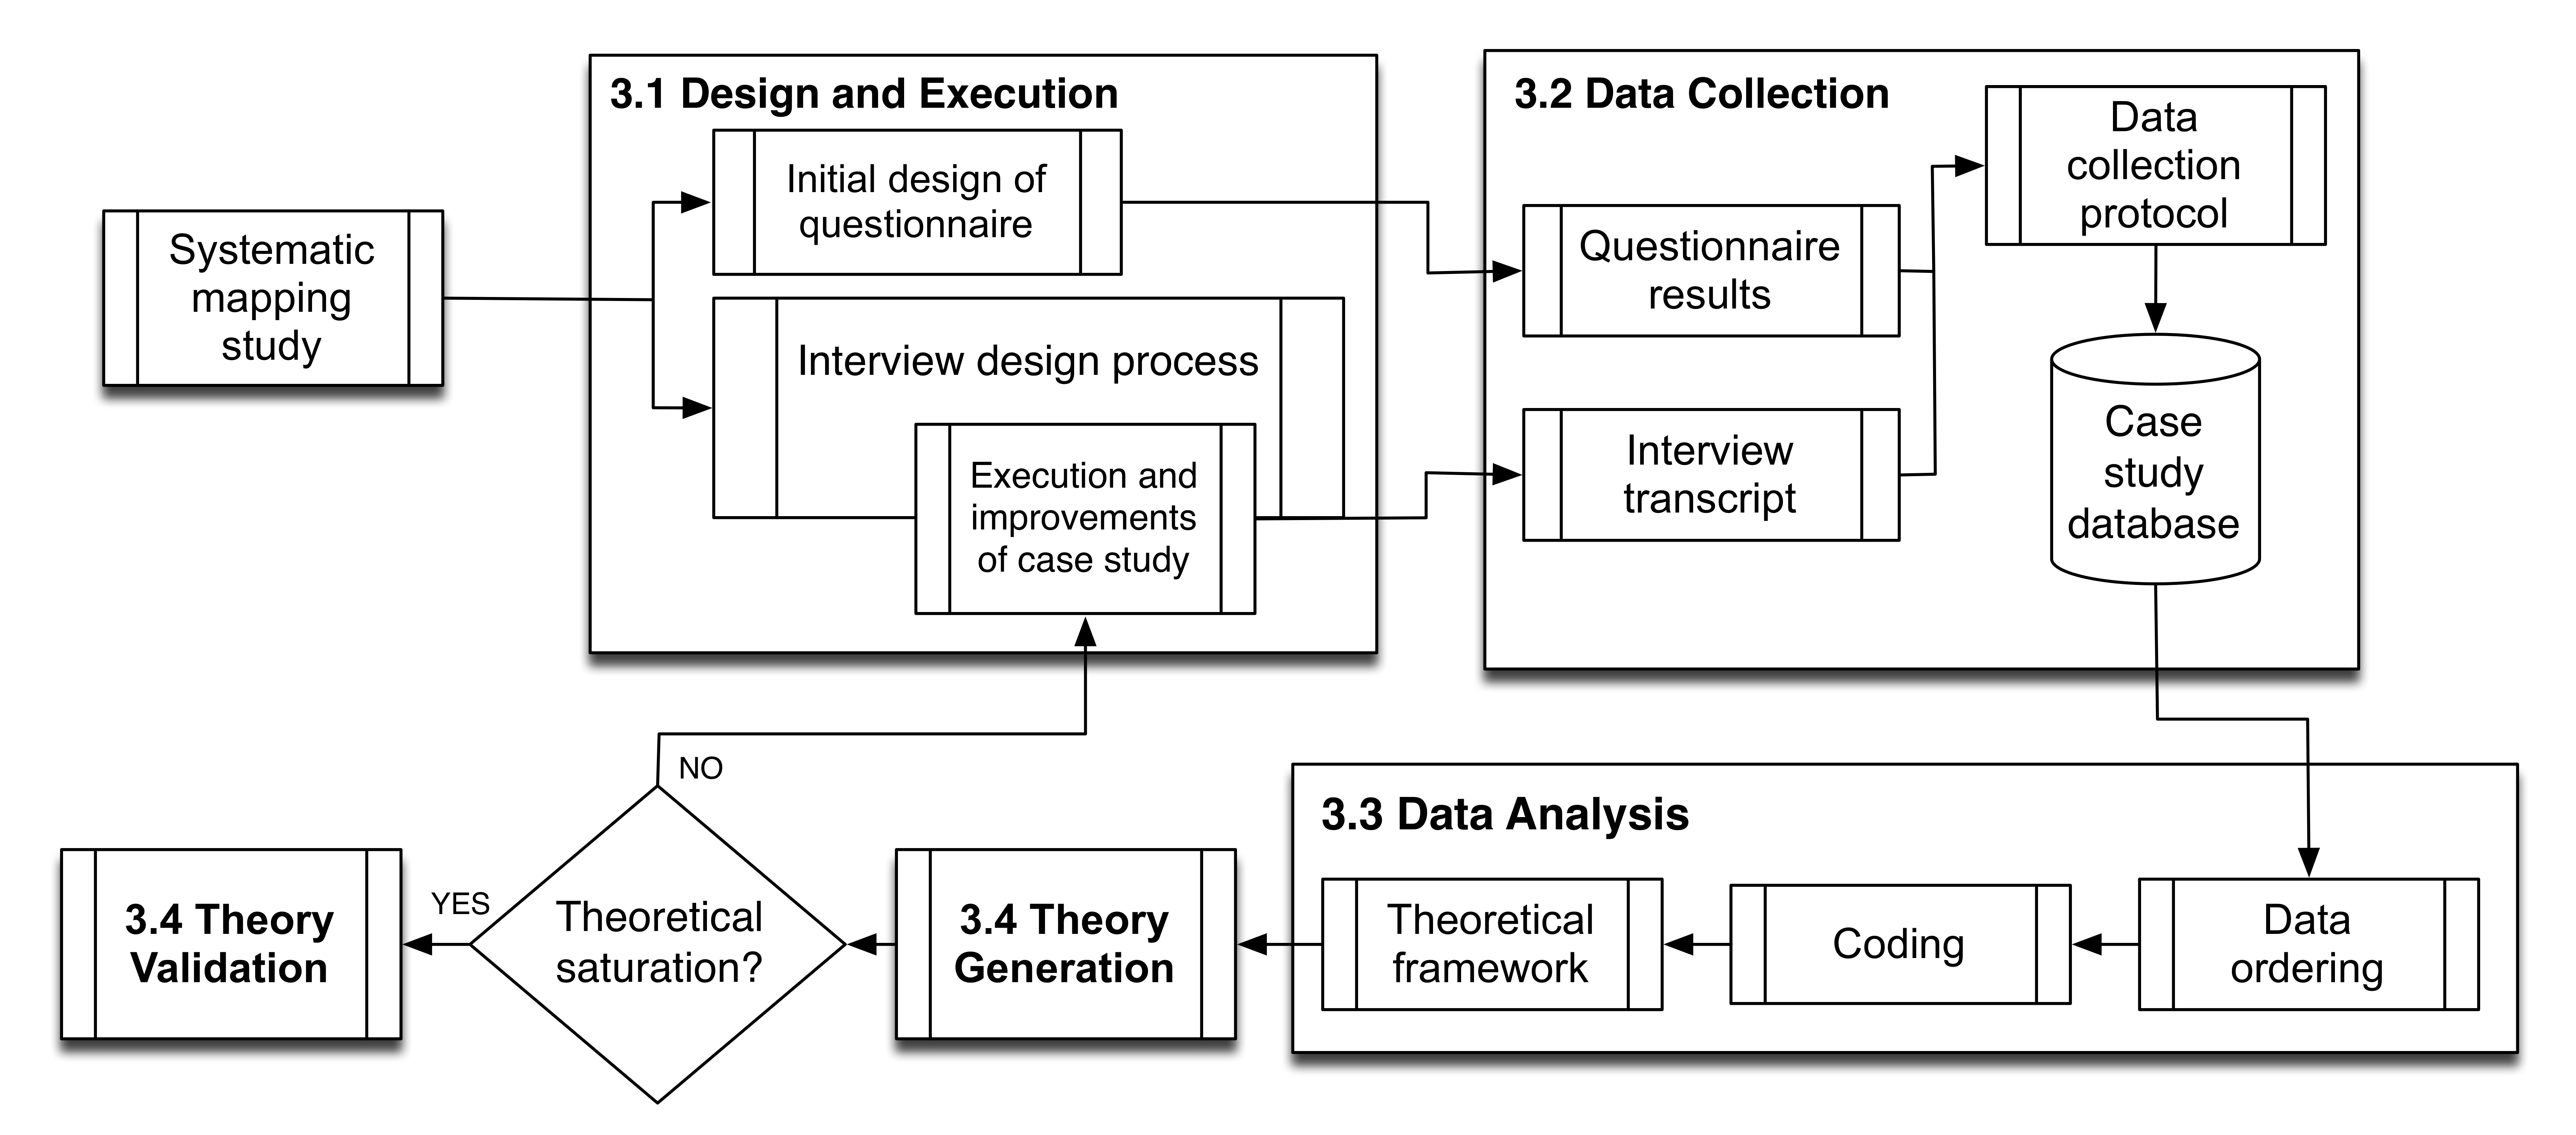
\includegraphics[width=4in]{figures/completemethodology2}
\caption{Grounded theory study process overview}\label{fig:gt:completemethodology}
\end{figure*}
%MUN: I think you can increase the font size in the figure a bit. Try thereby to keep the 
%height of the figure, expanding however the width (use horizontal space since it is a two 
%column figure). Change also in figure:
% - Write "Data Analysis" horizontally
% - Change names of macro-phases to upper-case, i.e. Design and Execution, Data Collection, Data Analysis, etc.
% - Add section number to macro-phase name, i.e. 3.1 Design and Execution, 3.2 Data Collection
% - Change "Discussion and Validation" into "Theory Validation" as you name it in the text.
% Also, add a section (3.5) that describes shortly what you did in "Theory Validation"


The aim of this research is to \textit{understand how software development strategies are engineered by practitioners in startup companies in terms of level of: structure, planning and control of software projects, in the period of time  that goes from idea conception to the first open beta release of the software product} \footnote{The above mentioned goal is structured according to the GQM paradigm \cite{Basili1992}.}.

Initially the boundaries of the research domain were set by means of non-systematic literature survey, which provided the initial keywords used further in the research process. Moreover it helped us in defining the research questions (RQs):


\begin{compactitem}

\item RQ-1 : What is the current state-of-practice related to software development strategy in early-stage startups?
\begin{compactitem}

\item RQ-1.1 : How do startups structure and execute the main engineering activities?
\item RQ-1.2 : How are product quality attributes considered by startups?
\end{compactitem}

\end{compactitem}

We investigated the software development approach undertaken by practitioners of startups.  Following a \textit{Grounded Theory} (GT) methodology \cite{Glaser1978}, we executed 13 semi-structured interviews integrated with follow-up questionnaires. From this, we elaborated and extracted the Green-field startup model (GSM) explaining the underlying phenomenon of software development in startups.

\textit{Grounded Theory} methodology is described by Robson as \textit{``the best approach to answer the question - What is going on here?''} and defined by its creators \cite{ColinRobson2009} as \textit{``a set of well-developed categories ( e.g. themes, concepts ) that are systematically interrelated through statements of relations to form a theoretical framework that explains some relevant social, psychological, educational, nursing or other phenomenon''} .

Despite GT has its roots in the social sciences, it has been increasingly used by Information System researchers and has been almost ignored by the SE research \cite{Coleman2007}. In 1997 Bertelsen advocated for a need of more qualitative research in SE \cite{Bertelsen1997}, and in the last decade we assisted to an increasing number of publications that used a GT-like approach in SE \cite{Coleman2008a,Coleman2007, Sulayman2012}.

Following the GT principles we attempted to capture the most relevant aspects of software development from startup practitioners, letting a theory emerge from the interviews and adjusting the research hypotheses and questions as we proceeded through. During these interviews we collected data related to engineering activities undertaken by startups in the time frame between the idea conception and the first open beta release of the product.  Then, we proceeded to the analysis of the data, finding important relations among concepts with a formal approach.

As suggested by Coleman, in view of the different versions of GT which emerged in the last years, researchers should indicate which \textit{``implementation''} of the theory is being used \cite{Coleman2007}. After the methodology was initially introduced, its original authors  had divergences regarding how the theory should be formed by analyzing the data (Strauss and Corbin on one side, Glaser on the other).  Glaser advocated for a more \textit{puristic} approach, where the theoretical categories should \textit{``naturally emerge from the data''}, whilst Strauss and Corbin formulated an updated version of the methodology, which leaves to the researchers an higher degree of freedom. The latter approach empowers researchers' \textit{``theoretical sensitivity''} \cite{Corbin1990}, and encourages them to outline the research problem beforehand. Since the knowledge obtained from parallel execution of the SMS \cite{SMS} and our direct experience with startups companies provided 
a good initial level of knowledge, in this study we use the Corbin and Strauss approach \cite{Strauss1998}.

In this research we address technical aspects related to software development in startups, exploring their operational dynamics. In view of the lack of agreement on an unique definition of the word \textit{startup}, we delimited our initial contextual boundaries to newly created innovative and single-product software companies, in the time-frame that goes from the idea conception to the release of the first product in highly scalable markets. Moreover, since most startups are web-oriented companies \cite{tc-webstartups-link, Allen2003}, in our case study, we inquired web companies with little or no operating history.

A complete overview of the overall case study methodology and execution is shown in Figure \ref{fig:gt:completemethodology}, which presents how we tailored the general GT methodology to our specific needs.


The initial design of the case study is supported by the results of the \textit{Systematic Mapping Study} (SMS) \cite{SMS} which contributed to define the initial questions for both questionnaires and semi-structured interviews. The process depicted in Figure \ref{fig:gt:completemethodology} is evolutionary and affects the design at each new iteration. In \textit{Data Collection} the empirical results are integrated and stored in a single case study database and subsequently processed in \textit{Data Analysis} to form the theoretical categories.  At each iteration the new emergent theory is updated following a formal procedure (\textit{Theory Generation}), and after verifying that \textit{Theoretical Saturation}\footnote{The point at which executing more interviews wouldn't bring any additional value for constructing the theory.} of categories has been achieved, we finally proceeded to \textit{Theory Validation}. 

The whole procedure has been executed simultaneously in pair on the same screen by the first two authors, handling conflicts by reviewing the rationale of decision with the third and fourth authors. When necessary we performed an in-depth review of the design of the research and data collected during the execution process. 

The process details are described in the following subsections, structured according to the five macro phases depicted in bold in Figure \ref{fig:gt:completemethodology}.



%--------------------------------------------------------------------------------------------------------------------------------------------------------------------------------------------------------------------------------%
\subsection{Design and Execution}
\label{desex}


This case study started based on a SMS of the literature regarding software development in startups \cite{SMS}. By means of this SMS we refined our research questions. The research questions have been narrowed down to outline the domain of our study, even though still broad enough to allow emerging new theories and to adjust the scope of the research \cite{Corbin1990}. 

The sampling of candidate companies took place in two distinct phases. At first we executed an initial convenience sampling \cite{Dawson2009}, which led to the identification of eight companies. Then we included five additional startups during the theory formation process (theoretical sampling) iteratively improving the sample according to the emerging theory. The characteristics of the sampled companies are reported in Table \ref{t_interviews-stats}. 


\begin{table*}[!t]
\renewcommand{\arraystretch}{1.3}
\caption{Companies overview} 
\label{t_interviews-stats}
\centering
\begin{tabular}{|c||c||c||c||c||c|}

\hline
    ID  &  Company age & Founding & Initial & Current & First product  \\
          &   (months)   & team   & developers  & employees      &  building time    \\
                    &      & &   &  & (months)   \\
   \hline
C1    & 11    & 4     & 2     & 11    & 6   \\
C2    & 5     & 2     & 2     & 6     & 3      \\
C3    & 18    & 4     & 4     & 4     & 6      \\
C4    & 17    & 3     & 2     & 11    & 6     \\
C5    & 20    & 2     & 1     & 4     & 12   \\
C6    & 30    & 3     & 2     & 4     & 1      \\
C7    & 12    & 2     & 1     & 7     & 4      \\
C8    & 24    & 4     & 3     & 16    & 4    \\
C9    & 5     & 5     & 4     & 5     & 1     \\
C10   & 43    & 6     & 4     & 9     & 4      \\
C11   & 36    & 3     & 3     & 6     & 2     \\
C12   & 12    & 3     & 3     & 3     & 3      \\
C13   & 24    & 2     & 2     & 20    & 3     \\
 
\hline
\end{tabular}
\end{table*}

All companies, except C10, were founded within the last three years (2009-2012), %MUN: I've shortened the text and
%added absolute numbers. Is 2009-2012 correct?
by an average of 3 starting members, which were in majority developers. Moreover, the number of current employees shows how, to different degrees, companies expanded the initial teams. All companies, except C5, brought their first product to market in less than 6 months from the idea conception. The products consist of web-applications, launched in different nations and market sectors. The growing team size and the publicly available data suggest an healthy status of the businesses.

We executed the case study online, supported by tools for video conferencing, recording each complete session. The interview subjects were the companies' CEOs or CTOs. We followed a step-by-step workflow, consisting of the actual interview, collection of additional material, preparation of the customized follow-up questionnaire and the iterative adjustment of the interview package artifacts\footnote{The interview package and follow-up questionnaire has been released under MIT License \cite{MITLicense} and it is available for download on Github \cite{GitHubInterviewPackage}. We encourage anyone interested in pushing this work forward, to fork the repository and contribute to it. If used in a research context, please inform us in order to be able to track where and how the interview package has been used.}.

The follow-up questionnaires were designed to capture additional data, gather missing information and confirm interview results by triangulation. The questionnaires have been tailored to each startup, partially taking advantage of the repertory grid principles \cite{Edwards2009}. To obtain better chances of quickly obtaining responses, questionnaires have been sent to respondents immediately after transcribing the interview results. Two weeks after the conclusion of the last interview, we closed our follow-up questionnaires and collected the data. %MUN: I don't understand this: you
% collected the data from questionnaires after ALL interviews have been finished, but on the other hand you 
% said the overall process was iterative (data analysis and triangulation let themes emerge which in turn were used
% in subsequent interviews). 

%--------------------------------------------------------------------------------------------------------------------------------------------------------------------------------------------------------------------------------%
\subsection{Data collection}
The data collection was designed to allow triangulation, which integrates multiple data sources converging on the same phenomenon. After transcribing the interview, we extracted conceptual relations, integrating them with the questionnaire's results. A well structured case-study database allowed us to easily retrieve and seek for information, assembling the evidence from the case study reports, as described also in \cite{Yin1994}. The database has been stored and constructed using the qualitative data analysis software package AtlasTI\footnote{Available online at \url{http://www.atlasti.com/} .} - one of the most suitable tools for GT \cite{Coleman2007}. 
We overlapped interviews with questionnaire results to adjust the data collection and take advantage of emergent themes and reveal possible inconsistencies. The data was analyzed simultaneously and with flexibility in mind in such a way that adjustments were made according to the emerging findings.
%--------------------------------------------------------------------------------------------------------------------------------------------------------------------------------------------------------------------------------%
\subsection{Data analysis}
Before starting the analysis, a data ordering procedure was necessary since interviews were spread across a multitude of topics. Therefore transcripts have been structured in thematic areas accordingly to different topic cards used during the interviews. We proceeded horizontally between same thematic areas of transcripts to be able to identify a better number of similar concepts, rather than going through an entire transcript at one time.

Once the data were ordered, we executed the process of coding interviews, following the steps listed below: 


\begin{compactitem}

\item Labels were assigned to raw data, and a first low-level conceptualization was carried out using both in-vivo and open coding \cite{ColinRobson2009}.
\item Concepts were grouped together into theoretical categories and subcategories. By means of axial coding we first described the different relations between subcategories, and then relations between subcategories and categories.
\item Categories were refined several times in the attempt to create different levels of abstraction and adjusting concepts, aided by a simple knowledge management tool.
\item Consistency among categories was validated by exploring and analyzing links among subcategories by means of selective coding.
\item The core category - the one with the greatest explanatory power -  was identified by analyzing the causal relations between high-level categories.
\end{compactitem}


During data extraction we used the technique of in-vivo coding since \textit{``direct quoting from the transcript gives more expressive power to the data''} \cite{ColinRobson2009} combined with the more descriptive procedure of open coding. Following the example of other grounded theories, developed in related areas such as Information Systems \cite{Orlikowski1993} and Software Process Improvement \cite{Coleman2006}, we performed the high-level conceptualization during creation of categories, in the process of refining axial and selective coding.

As we were iterating through the interviews, we analyzed new data accordingly, by updating codes and categories on necessity, and taking notes in the form of memos to adjust the new emerging theory. To improve the speed of the coding process, we analyzed all the transcripts one part at-the-time: transcripts followed the semi-structured interview format, and this approach enhanced the chances of finding similar codes across different transcripts, allowing us to quickly iterate and update categories.

Given the large number of codes, categories, properties, propositions and related questions that evolved from the analytical process \cite{Corbin1990}, an important activity that helped the coding process was memoing. It constituted an important component involved in the formulation and revision of theory during the research process. For this purpose we made use of three different types of memos: code memos, theoretical memos and operational memos. The first type of memo is related to the conceptual labeling of open codes, whilst the second type concerns axial and selective coding, and thus focusing on paradigm features. Finally, operational memos contain directions relating to the evolving emerging theory.

After the coding process the first representation of the experience map identified in GT is constructed by means of a theoretical framework. The theoretical framework is presented in the form of a network of categories and subcategories that are linked together according to cause-effect relationships \cite{Corbin1990}. During the formation of the theoretical framework the researchers operated by means of a  bottom-up approach. From the empirical data and coding process, the framework developed into two different levels: a detailed level representing the network of subcategories (identified mainly by the axial coding process), and a high-level representation of the main categories network (identified mainly by the selective coding process).

%--------------------------------------------------------------------------------------------------------------------------------------------------------------------------------------------------------------------------------%
\subsection{Theory generation}

As mentioned in Section \ref{desex}, emergent theories have been tested by integrating additional companies into the sample, selected following the principle of theoretical sampling \cite{Yin1994}. 

The process of theory generation took place at each iteration together with interview execution, where we systematically analyzed the theoretical framework by means of the paradigm model introduced by Corbin \cite{Corbin1990}. The paradigm model is composed by: 

\begin{compactitem}
\item \textit{Causal conditions}: the events which lead to the occurrence of the phenomenon, that is our core category
\item \textit{Context}: set of conditions in which the phenomenon can be extrapolated
\item \textit{Intervening conditions}: the broader set of conditions from that the phenomenon can be generalized
\item \textit{Action/interaction strategies}: the actions and responses that occur as the result of the phenomenon
\item \textit{Consequences}: specification of the outcomes, both intended and unintended of the actions and interaction strategies
\end{compactitem}

Within the limits of the critical bounding assumptions, the role of the generated theory is to explain, predict and understand the underlying phenomenon.

\subsection{Theory Validation}
%MUN: put here what I wrote in the comment in Section "Theory validation" (i.e. the section following the GSM)

%--------------------------------------------------------------------------------------------------------------------------------------------------------------------------------------------------------------------------------%

\section{Results: Green-field startup model}
\label{res:gsm}

By analyzing the interview transcripts with the GT process we extracted the information necessary to form the theoretical model. The initial coding process (open and in-vivo) provided 630 unique codes \footnote{Available at \url{https://github.com/adv0r/BTH-Interview-Package}.}, grounded to 1295 citations in the transcripts, divided according to the thematic areas. The thematic areas were divided according to the development phases designed for the interview process. The raw codes constitute the empirical foundation of the theoretical categories, which has been used to form the Green-field startup model (GSM).

The GSM captures the underlying phenomenon of software development in early-stage startups. The framework is formed by 128 sub-categories, clustered in 35 groups, and finally in 7 categories at the highest level of abstraction. By the means of the GSM we provide explanations of the development strategies and engineering activities undertaken by startups.
%--------------------------------------------------------------------------------------------------------------------------------------------------------------------------------------------------------------------------------%
\subsection{Framework overview}
\label{res:gsm:frmov}
The main concepts representing the underlying phenomenon have been grouped together to form high-level categories. Figure \ref{fig:gsm} shows the network of causal relationships (represented by arrows) between categories (represented by blocks). Each node is linked to subsequent nodes which are called successors, and preceding nodes, called predecessors. The relations between them are denoted by the direction of the interconnecting arrows. The network is read from left to right.

\begin{figure*}[!t]
\centering
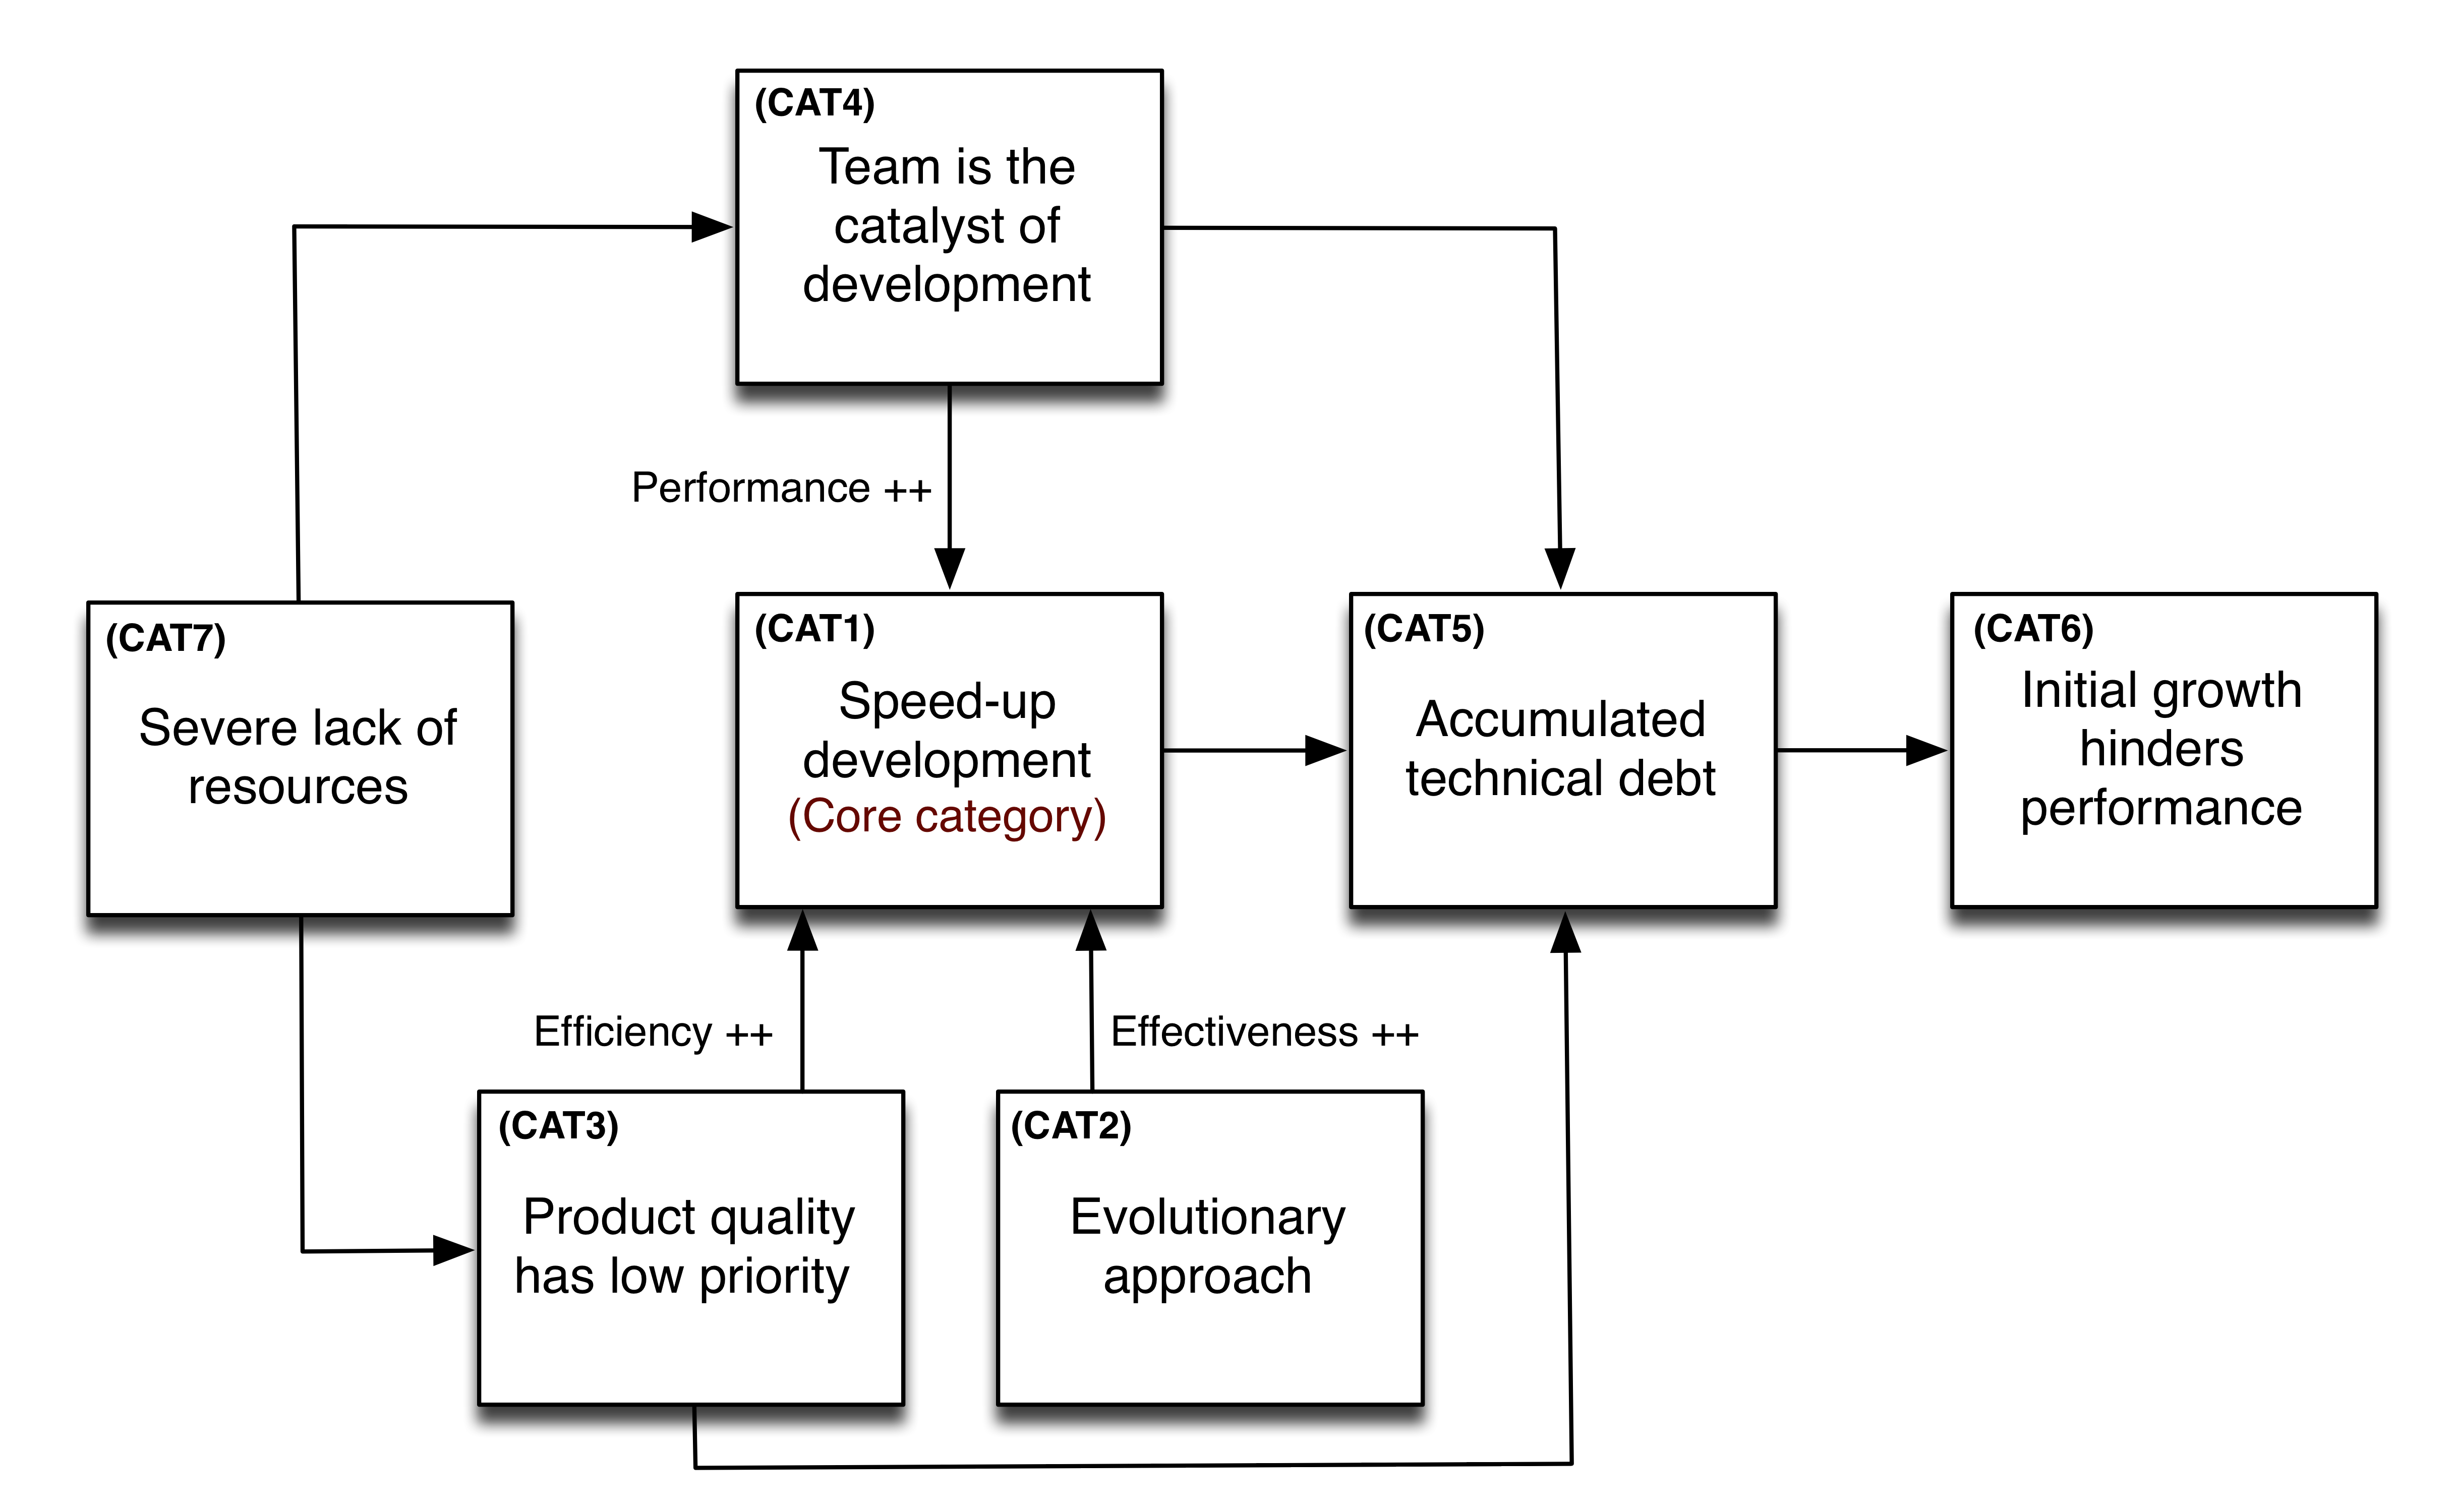
\includegraphics[width=4in]{figures/high-level}
\caption{Green-field startup model}\label{fig:gsm}
\end{figure*}

In forthcoming the explanation of the GSM we emphasize labels of theoretical categories using the \textit{italic} font style. For the main categories shown in Figure \ref{fig:gsm}, when necessary we also make use of identifiers (i.e. CATx) to facilitate the reading of this section.
The network is centered around the core category, \textit{speed-up development}, which is the most interconnected node in the framework reflecting the fact that \textit{``it is the one (category) with the greatest explanatory power''}  \cite{Strauss1998}. The meaning of the labels on the three arrows that reach the core category (efficiency, effectiveness and performance) is discussed in detail in section \ref{valt}. %MUN: this refers to the validity threats section. Do you mean rather the "Theory Validation" section?

A contextual condition which characterizes, to some extent, each and every startup, is the \textit{severe lack of resources}. In fact, the capabilities of an early-stage startup to support its development activities are constrained by an extremely limited access to human, time and intellectual resources, eventually leading to a general absence of structures and processes.

The \textit{severe lack of resources} forces the company to focus on implementing an essential set of functionalities and it is one of the main reasons why the \textit{product quality has low priority} respect to other more urgent needs\footnote{There are some exceptions where the quality aspects actually matter and such cases will be discussed in section \ref{valt} %MUN: this refers to the validity threats section. Do you mean rather the "Theory Validation" section?
.}. At the same time, to be able to deal with such constraints, startups must depend on a small group of capable and motivated individuals.

As it has been unanimously expressed by respondents, from a software perspective, the most urgent priority is to \textit{speed-up the development} as much as possible by adopting an extremely flexible and effective \textit{evolutionary approach}. On the other hand the efficiency of teamwork is facilitated by the low attention initially given to architectural aspects related to product quality. This allows startups to have a faulty but functioning product, which can quickly be introduced to the market beginning with the in-house implementation of the prototype from day-one.

The initial employees are the ingredients which enable high levels of performance in software development. To support a fast-paced production environment, engineers are required to be highly committed, co-located, multi-role, and self-organized. In other words \textit{team is the catalyst of development}.
With an essential and flexible workflow, which relies on tacit knowledge instead of formal documentation, startups are able to achieve very short time-to-market cycles. However, each line of code, written without following structures and processes, contributes to grow the \textit{accumulated technical debt}, which is further increased by having almost non-existing specifications, a minimal project management and a lack of automated tests.

Despite the fact that the consequences of such debt are not clearly perceived in the initial stages (where finding the product/market fit as quickly as possible is the most important priority), startups, which survive to subsequent phases, will likely increment their user-base size, the product size, and the number of developers. This will require the company to eventually pay the \textit{accumulated technical debt}, confronting the fact that an \textit{initial growth hinders productivity}.

In the following subsections we are going to explain in detail all the categories presented in Figure \ref{fig:gsm}, and conclude in subsection \ref{res:gsm:th} with the final theory. In the explanations we use identifiers of the companies presented in Table \ref{t_interviews-stats} (i.e. Cx) to highlight statements recorded from the interviewees.

%--------------------------------------------------------------------------------------------------------------------------------------------------------------------------------------------------------------------------------%
\subsection{Severe lack of resources}
\label{res:gsm:cat7}
The concept of \textit{severe lack of resources} characterizes the uncertainty of the development strategies in startups and it is composed by three subcategories: \textit{time-shortage}, \textit{limited human resources} and \textit{limited access to expertise}.


Since startups want to bring the product to market as quickly as possible, the resource they are the most deprived of is time. Startups operate under a constant time pressure, mainly generated by external sources (\textit{investor(s) pressure}, \textit{business pressure}) and sometimes internal necessities such as \textit{internal deadlines} and \textit{demo presentations at events}. In this regard, C3 commented: \textit{``Investors wanted to see product features, engineers wanted to make them better. Finally the time-to-market was considered more important and the team interests was somehow sacrificed.''}

In addition, to compensate the \textit{limited human resources},  practitioners need to empower \textit{multi-role and full stack engineers}, as confirmed by C1: \textit{``Everyone was involved in any tasks, from mobile to web development, organizing themselves in choosing the part to implement''}.

The extent to which startups have access to specialized knowledge - both internal and external to the company - is extremely reduced when compared to traditional established software companies. Therefore, in order to partially mitigate the \textit{limited access to expertise}, startups rely on the external aid of mentors or advisors. Under these strict limitations, most of the decisions related to software development are fundamentally trade-off situations (confirming Himola's results \cite{Hilmola2003}).
%--------------------------------------------------------------------------------------------------------------------------------------------------------------------------------------------------------------------------------%
\subsection{Team is the catalyst of development}
\label{res:gsm:cat4}
Among the different aspects fostering the speed of the development process, the startups' main focus is on the characteristics of the initial team.

In startups \textit{developers have big responsibilities}. In fact, the \textit{limited human resources}, discussed in CAT7, cause the team-members to be active in every aspect of the development process, from the definition of functionalities to the final deployment.

Early engineers in the founding team of a startups are typically \textit{multi-role and full-stack engineers}: they are full-stack for being able to tackle different problems at different levels of the technology stack (\textit{generalists developers instead of specialists}) and multi-role since usually \textit{engineers are responsible for marketing/sales/development}. As remarked by  C11: \textit{``Instead of hiring gurus in one technology, startups should hire young developers, generalists, that know how to quickly learn new technologies, and quickly move among a huge variety of tasks.''}

Moreover, having a \textit{very small and co-located development team} enables members to operate with high coordination, control and communication, which heavily rely on \textit{tacit knowledge},  replacing most of the documentation with informal discussions. Practitioners reported that keeping the development team small helps startups in being fast and flexible, as remarked by C8: \textit{``If you have more than 10 people, it is absolutely impossible to be fast''}. Then, also \textit{previous working experience} and \textit{knowing each other before starting the company} enforce the efficiency of activities by \textit{limiting the need of formalities between team-members}.

In every software company, \textit{skilled developers are essential for high speed} in development. Especially in startups, the ``hacking culture'' and a tendency to the ``just-do-it'' approach allow the team to quickly move from the formulation of a feature idea to its implementation. In this regard, C1 comments: \textit{``We had a hacker culture/environment, people hacking stuff without formally analyzing it, but breaking it down and finding a way around. Ticket on trello and go.''}  

A \textit{limited access to expertise} forces the team to rely mainly on their personal abilities, even though asking opinions to mentors is reported to be a viable practice to maintain feasible objectives. Furthermore \textit{teams work under constant pressure}, \textit{``up to 16 hours per day''}, %MUN: add Cx to this statement since it is a citation?
mainly constrained by a tight \textit{time shortage}.

Finally, startups present founders-centric structures, and especially in the early-stage, it is clear that \textit{CTO/CEO background has high-impact} on the company's development approach. For instance, in case of an academic background, the CTO encourages the introduction of some architectural design before the development phase. Moreover, even though the CTO/CEO starts guiding initially the development process, most of the decision are taken consensually by all members of the team. Then, the CTO/CEO decides only in particular situations where some conflicts occur.
%--------------------------------------------------------------------------------------------------------------------------------------------------------------------------------------------------------------------------------%
\subsection{Evolutionary approach}
\label{res:gsm:cat2}
Among different approaches to development, startups prefer to build an initial prototype and iteratively refine it over time, similarly to the concept of \textit{``evolutionary prototyping''} \cite{EvProt}.  The reason of using this approach is that startups want to validate the product against the market as soon as possible, finding the proper product/market fit. Indeed, they can focus on developing only parts of the system they want to validate instead of working on developing a whole new system. Then, as the prototype is released, users detect opportunities for new functionalities and improvements, providing their feedback to developers.


Since \textit{flexibility and reactiveness are the main priorities}, the most suitable class of software development approaches are clearly highly evolutionary in nature. In fact, as \textit{uncertain conditions make long-term planning not viable}, startups cannot base their work on assumptions without rapidly validating them, releasing the product to market. The uncertainty is first of all in the team composition. Since the teams are typically very small and the project knowledge is not documented, even a little change in their composition (e.g. a developer falls ill) can have a very high impact on the overall product development. Furthermore, startups operate in a continuous evolving environment in terms of competitors and targeted market sectors. Then, to obtain a competitive advantage in the market, startups typically make use of cutting-edge solutions, characterised by an evolution that cannot be foreseen in the long run. However, a special role in daily decisions is covered by user feedback 
and requests, which represent the main drivers for defining the product features in the short-term.

To obtain fast user responses and quickly \textit{validate the product}, startups \textit{build a functioning prototype and iterate on it} over time. Paraphrasing C4, \textit{``[\ldots] you should start with something that is really rough and then polish it, fix it and iterate. We were under constant pressure. The aim was to understand as soon as possible the product market/fit iterating quickly, adjusting the product and releasing fast.''}

The companies focus on building a small set of functionalities to include in the first version, and \textit{progressively roll-out to a larger number of people} with very \textit{small iterations} (confirmed again by C4: \textit{``we deploy from 5 to 20 times a day''}).

The objective of this evolutionary approach is to avoid wasting time in ``over-engineering the system'' and building complex functionalities that have not been tested on real users. By releasing a very small number of good-enough functionalities (see CAT3) the startup can verify the suitability of the features and understand how to adjust the direction of product development towards actual users' needs. The first version of the product is typically a prototype which contains the basic functionalities developed with the least possible effort that can validate critical features, enabling the startup's survival in the short term (recalling  Ries' definition of \textit{Minimum Viable Product} (MVP) \cite{Ries2011}).

Supported by \textit{direct contact and observation of users}, \textit{automated feedback collection} and \textit{analysis of product metrics}, startups attempt to \textit{find what is valuable for customers} with activities in agreement with Blank's \textit{Customer validation} stage \cite{Blank2005}.

%--------------------------------------------------------------------------------------------------------------------------------------------------------------------------------------------------------------------------------%
\subsection{Product quality has low priority}
\label{res:gsm:cat3}
The interests of software startups, related to the product, are mainly concentrated on building a  \textit{limited number of suitable functionalities} rather than fulfilling restrictive non-functional requirements. This strategy allows them to quickly release simple products with less need of preliminary architectural studies.


Exploring quality aspects considered during the development process, the only important concerns are expressed towards the user experience\footnote{According to the ISO 9241-210 (Ergonomics of human-system interaction), UX is defined as \textit{``a person's perceptions and responses that result from the use or anticipated use of a product, system or service''.} Even though this definition leaves so much to interpretation, we can refer to it as presented in the glossary.}, in terms of \textit{ease of use, attractiveness of the UI} and most of all, \textit{smooth user-flow without interruptions}. The fact that \textit{UX is the only important quality} is remarked by C11: \textit{``When a user needs to think too much on what action should be done next, he will just close the application without returning''} and confirmed by C3: \textit{``If the product works, but it is not usable, it doesn't work''.}

The extent to which quality aspects are taken into account might heavily depend upon the market sector and the type of application. Nevertheless, realizing high level of UX  is often the most important attribute to consider for customer discovery of  evolutionary approaches in view of the \textit{limited human resources} and \textit{time shortage}, presented in CAT7. C4 confirms: \textit{``None of the quality aspects matter that much as the development speed does.''}

To achieve a good level of UX while dealing with lack of human resources and time shortages, startups can analyze similar products of bigger companies which can afford more rigorous usability studies. Then, the users' feedback and product metrics begin to have a central role in determining the level of UX achieved. Product metrics are typically web-based \textit{statistical hypothesis testing}, such as A/B testing. %MUN: add reference or explain shortly what A/B testing is

Other than UX, some other factors can influence the quality concerns of development:


\begin{compactitem}

\item The \textit{efficiency emerges after using the product}, letting engineers avoid wasting time in excessive improvements of not-validated functionalities. The level of efficiency can be optimized after attesting the effectiveness of the minimal set of functionalities, obtained according to CAT2 and to the concept of MVP.
\item The \textit{product should be reasonably ready-to-scale} to be able to accommodate a potential growth of the user-base\footnote{Note that startups tackle fast growing markets which are particularly subject to sudden user growths}. Thanks to modern cloud services, startups can \textit{externalize complexity to third party solutions} achieving a good level of scalability with a reasonable effort.
\item Realizing high reliability is not an urgent priority since \textit{users are fault-tolerant in innovative beta products}. In these cases, users have typically a positive attitude towards the product, even though it presents unreliable behaviours. In this regard, the main focus of beta testing is reducing frictions between the product and the users, often incorporating usability testing. In fact, the beta release is typically the first time that the software is available outside of the organization that developed it. \footnote{Detailed discussion of the impact of innovative products on the user satisfaction is presented in Appendix according to the Kano model.}.
%MUN: do you use the Kano model in Theory Validation? Change text to refer to the correct section.
\end{compactitem}


Finally, startups implement a \textit{limited number of suitable functionalities}, which in view of \textit{limited human resources} and \textit{time shortage}, represent a viable strategy to focus on shortening time-to-market.%--------------------------------------------------------------------------------------------------------------------------------------------------------------------------------------------------------------------------------%
\subsection{Speed-up development}
\label{res:gsm:cat1}
As remarked initially, \textit{speed-up development} represents the core category of the GSM. Firmly grounded as the primary objective of startups, it shows the most important characteristic of developing software in the early stage.


As mentioned before, in order to \textit{speed-up development}, startups adopt evolutionary approaches supported by a solid team focusing on implementing a minimal set of suitable functionalities. Startups \textit{keep simple and informal workflows} to be flexible and reactive, adapting to the fast changing environment. While a rigorously defined workflow generally consists of an established sequence of well-defined steps to follow, startups, by contrast, adopt informal workflows. This choice is mainly dictated by contextual factors characterized by the general conditions of unpredictability and uncertainty. The adoption of informal workflows is facilitated by the fact that teams are typically self-organized and \textit{developers have big responsibilities} .

Additionally, possible planning activities are refrained by the aim to shorten time-to-market, as reported by C8: \textit{``Speed was the essence so we didn't plan out too many details''}. To deal with such unpredictability, startups prefer to take decisions as fast as possible, mainly by means of informal and frequent verbal discussions.

Despite Agile principles appear to be suitable to embrace changes, especially in the early-stage, development practices are often perceived as time-wasters and ignored to accommodate the need of releasing the product to market as quickly as possible. In this regard, to maintain the simplest and most informal approach, startups aim to \textit{find the product/market fit quickly} and implement a \textit{limited number of suitable functionalities}. This approach is considered possible also in view of a lack of systematic quality assurance activities, since only the user experience is considered as important and other quality aspects, such as efficiency, can be postponed after the first release.  

Another strategy, which supports startups in quickly delivering products, is the \textit{externalization of complexity on third party solutions} by: making use of third party components (COTS) and open source solutions (both for product components, and development tools and libraries); taking advantage of  external services; and deploying the product on external infrastructures, for the sake of delivering a \textit{product reasonably ready to scale} for a possible future growth.

Even though \textit{the use of well-integrated and simple tools} allows startups to automate many activities and reduce their completion time, drawbacks of such approaches are the increased concerns of interoperability issues. A category of tools is represented by advanced version control systems, which are not only used to manage the code-base, but for many other purposes such as: assigning tasks; trace responsibilities; configuration management; issue management; automatic deployment; discussions and code reviews.

Startups can further improve development speed by making \textit{use of standards and known technologies} which are widely recognized, well tested, and supported by strong communities. Moreover, the use of widely adopted standards and frameworks reduces the need of a formal architectural design since most of implementation solutions are well documented and ready-to-use. This is confirmed by C1: \textit{``as long as you use Ruby standards with the Rails framework, the language is clean itself and doesn't need much documentation''.}

Other important factors that positively impact the speed of development are the team's desire to: \textit{create disruptive technologies}; to \textit{demonstrate personal abilities}; and to \textit{have the product used in the market}. As reported by practitioners, these factors are essential to enhance the morale of developers and therefore to achieve higher team performances. By contrast, especially in the typical sprint-based environments of Agile, when a developer is not \textit{able to meet deadlines} the morale goes down, hindering the development speed.

Finally the constant pressure under which the company regularly operates, leads the team to often \textit{work overtime to meet deadlines}. But as reported by practitioners, such way of working can be an effective strategy only in the short term since it can lead to poorly maintainable code and developer burnouts in the long run.
%--------------------------------------------------------------------------------------------------------------------------------------------------------------------------------------------------------------------------------%
\subsection{Accumulated technical debt}
\label{res:gsm:cat5}
Startups achieve a very high development speed by radically ignoring aspects related to documentation, structures and processes. However, although these aspects are not considered important in the very first stages, they will become increasingly more important for the productivity in the long-term, as we illustrate in CAT6.


Instead of traditional requirement engineering activities, startups make use of \textit{informal specification of functionalities} by means of ticked-based tools to manage low-precision lists of features to implement, written in form of self-explanatory user stories \cite{AgilePlan}. Practitioners intensively use physical tools such as post-it notes and whiteboards, which help in making functionalities visible and prioritizing stories based on personal experiences. C4 comments \textit{``[\ldots] it is the only way. Too many people make the mistake of sitting down and write big specs and then they build it for four months, realizing the product is not valuable only at the end.''}

Since startups are risky businesses by nature, even less attention is given to the traditional phase of \textit{analysis}, which is replaced by a \textit{rough and quick feasibility study}   \textit{``only sometimes and however informally''}, as stated by C5.  First of all it is generally \textit{hard to analyze risks with cutting-edge technologies}. To find out the feasibility of such cutting-edge projects, startups attempt a first implementation with rough and informal specifications, assuming that project's complexity will remain limited to a small number of functionalities, as discussed in CAT3. Additionally by \textit{keeping the product as simple as possible} and learning from competitors' solutions and mistakes, practitioners can use their \textit{past experiences in similar contexts to help assessing feasibility} of the project. Finally, to avoid restrictions on the flexibility of the team, potential limiting decisions are taken only when strictly necessary and anyhow as late as possible.

Another important factor which contributes to \textit{accumulate the technical debt} is the general \textit{lack of architectural design}, substituted by \textit{high-level mockups and low-precision diagrams}, \textit{using modularization and frameworks from day 1} and \textit{describing critical interactions with third-party components only}. In particular, the use of well-known standards, frameworks and conventions limits the need of formal UML \cite{UML} diagrams and documentation, and provide a minimum level of maintainability costs. Additionally, since quality aspects are not a main concern (see \textit{limited number of functionalities} and \textit{efficiency emerges after using the product} in CAT3) having a well-structured architecture remains a secondary priority, and design is conducted only when strictly necessary.

A similar attitude towards verification and validation brings startups to a severe \textit{lack of automated testing}, which is mainly replaced by manual smoke tests executed by: trying the product internally; seeking for critical faults; and letting early adopters report non-critical bugs.  Paraphrasing C3, \textit{``Trying the product internally allows us to get rid of 50\% of bugs of important functionalities. Meanwhile users report bugs of secondary functionalities, eventually allowing us to mitigate the lack of testing. Indeed, staying one week in production enables us to identify 90\% of bugs''.} The lack of complete automated tests is partially also motivated by the fact that \textit{users are fault-tolerant in innovative beta products} and  by the limited number of functionalities, which allow the team to easily control critical bugs. However, in certain cases where components of the system might cause loss of data or severe damages to the product or users, engineers realize a reasonable level of 
automatic testing. In such cases, aided by modern automatic tools, they can quickly assess the status of the system integration as they add new functionalities to the product.

Furthermore, a rigid project management is perceived as \textit{``waste of time''} which hinders the development speed since the \textit{uncertainty makes formal scheduling pointless} (C9  reports that \textit{``initial chaos helps to develop faster''}). Startups' \textit{minimal project management}  is supported by keeping: \textit{internal milestones short and informal}, \textit{low-precision task assignment mechanism}  and a very low attention for project metrics (paraphrasing C13, \textit{``the only track of progress was made by looking at closed tickets''}). In this context \textit{only a final release milestone is viable}, which helps practitioners to remain focused on short term goals and put new features in production. To further \textit{speed-up development}, startups \textit{simplify issue management by integrating it with feature management}. Then, the \textit{limited number of functionalities} and the {use of standard/known technologies} with a \textit{simple workflow} are the main reasons for 
not establishing a heavy project management process since the project and technologies can be autonomously managed by the development team (with characteristics of: co-location, self-organization and very small size). %MUN: do you mean small team size?

Finally, one of the categories, which most contributes in growing the \textit{accumulated technical debt}, is the substantial  use of informal and verbal communication channels on a daily basis. The high co-location and the fast paced development approach increase the volume of \textit{tacit knowledge} and severe lack of any kind of documentation.  C4 observes in this regard that:  \textit{``[\ldots] the issue of having documentation and diagrams out of the source code is that you need to update them every time you change something. There is no time for it. Instead, there is a huge pay off in having a code that is understandable itself.''}
This approach is supported by the fact that startups make use of  \textit{simple and informal workflow}, \textit{standard/known technologies}, \textit{very small and co-located development team} with \textit{limited need of formalities}.
%--------------------------------------------------------------------------------------------------------------------------------------------------------------------------------------------------------------------------------%
\subsection{Initial growth hinders performance}
\label{res:gsm:cat6}
The lack of attention given in the first phases to engineering activities allows startups to ship code extremely quickly (see CAT5). However, if successful, the initial product becomes more and more complex over time, the number of users increases and the company size starts to grow. Under these circumstances the need of controlling the initial chaos forces the development team to return the \textit{accumulated technical debt} instead of focusing on new users' requests. Hence, \textit{initial growth hinders performance} in terms of number of new user stories implemented in a certain amount of time, which brings new suitable functionalities to the users.


When the number of users increases, customers become more quality demanding and also scalability issues start to arise. Usually, \textit{company and user size grow} when new business events occur, such as: a \textit{new round of funding}, a possible \textit{acquisition}, the release of a \textit{competing product on the market}, or when the project is \textit{open for the first public release}. As a consequence, the \textit{increasing number of users} creates a growing number of requests and expectations. Therefore, whereas the project lacks of minimal processes, suddenly, \textit{the current team is not able to manage increased complexity} of new functionalities to implement and maintain the codebase.

Subsequently, practitioners start considering the need of project management activities, also in view of \textit{hiring new staff members}, as discussed by C13: \textit{``(project management) is strictly necessary if you radically change the team or when the team grows.  The informal communication and lack of documentation slow down the process afterwards''}.  Project management becomes further important when the \textit{focus shifts to business concerns}. Part of the effort, which was initially almost entirely dedicated to product development, is required to move to business activities. Moreover the availability of project information becomes an important issue because of the accumulated \textit{tacit knowledge}, which hinders the ability of new hires to quickly start the development of project tasks.

When the company faces growth, the partial and informal engineering activities that have been conducted during the first phases of \textit{rush} development (refer to CAT5 subcategories \textit{minimal project management}, \textit{informal specification of functionalities}, \textit{rough and quick feasibility study}, \textit{lack of automated testing}, \textit{tacit knowledge}), force the company to \textit{pay off the accumulated technical debt}. Under these circumstances, startups need to be able to cope with the renewed needs and expectations of both the company (internal necessities) and customers (product).

Another factor that slows down performance is caused by the fact that \textit{portion of codes needs to be rewritten} and \textit{substantial refactoring of the codebase} is required by increasing product demands.

Practitioners realize that some decisions taken (or not taken) during the \textit{rough and quick feasibility study} before starting the implementation, have led to negative consequences on the long term performance and maintainability of the product. Additionally, the initial decisions of the product design might not be able to satisfy the increased demands of the product's users and developers (\textit{lack of architectural design}). The combination of these factors leads to the need of \textit{re-engineer the product}.

By re-engineering the systems, startups aim to \textit{increase the scalability of the product/infrastructure} and starting to \textit{standardize the codebase with well-known frameworks}.

C7 reports that: \textit{``To mitigate this (lack of frameworks) I had to make a schema for other developers when we hired them. We had to do a big refactoring of the codebase, moving it from custom php to Django, normalizing the model and making it stick with the business strategy. I had the code in different php servers communicating via JSON, some engineering horror. Now  that we are fixing it, it's really painful. We had to trash some code. However I don't regret that I didn't make this choice sooner, it was the only way''}.

The \textit{fear of changing a product, which is working}, arises when product complexity increases. The changes to the codebase, to support bug fixing, become highly interrelated with other functionalities and difficult to manage because the product is poorly engineered (see CAT5). Therefore, the fear arises from changing a validated product that might bring changes to the user responses.

The increasing number of feature requests causes the \textit{growing necessity of having a release plan}, rationalizing the rollout of new features.

Therefore, startups begin to \textit{partially replace informal communication with traceable systems} and \textit{introduce basic metrics for measuring project and team progress} in order to establish an initial structured workflow. In conclusion, because the increasing number of users causes issues in scalability and reliability, the \textit{need of more structured workflow} becomes of major relevance. C11 states: \textit{``Yet, it is still better to have a reasonable drop-down in performance when team grows than lose time in the beginning''}.
%--------------------------------------------------------------------------------------------------------------------------------------------------------------------------------------------------------------------------------%
\subsection{Theory}
\label{res:gsm:th}
In order to explain and understand the development strategies in early-stage software startups we construct the theory generated and supported by the above presented GSM:

\begin{theory}
Focusing on limited number of suitable functionalities, and adopting partial and rapid evolutionary development approaches, early-stage software startups operate at high development speed, aided by skilled and highly co-located developers. Through these development strategies, early-stage software startups aim to find early product/market fit within extremely uncertain conditions and severe lack of resources. Nevertheless, by speeding-up the development process, they accumulate technical debt, causing an initial and temporary drop-down in performance before setting off for further growth.
\end{theory}

As discussed in section \ref{valt}%MUN: this refers to the validity threats section. Do you mean rather the "Theory Validation" section?
, we formed the theory by applying the paradigm model, introduced by Corbin \cite{Corbin1990}. The theory is composed by different elements reflecting the paradigm model:

\begin{compactitem}

\item \textit{Causal conditions} are represented by three main conceptual categories: \textit{product quality has low priority}, \textit{evolutionary approach} and \textit{team is the catalyst of development}.
\item \textit{Phenomenon} is represented by the core category \textit{speed-up development}.
\item \textit{Context} is limited to web early-stage software startups operating in conditions of severe lack of resources aiming to early find product/market fit.
\item \textit{Intervening conditions} are  summarized by the extremely uncertain development environment.
\item \textit{Action and interaction strategies} are represented by the accumulation of technical debt.
\item \textit{Consequences} lead to a temporary performance drop-down.
\end{compactitem}

%--------------------------%%--------------------------%%--------------------------%%--------------------------%%--------------------------%%--------------------------%%--------------------------%
\section{Theory Validation}
\label{res:val}

In this section we discuss the validity of the GSM by means of cross-methodological observations:
%MUN: expand this discussion a bit (motivation why you do this like you do it) and move to Section 3.5. Then write here just that you perform theory validation as discussed in Section 3.5 (and remove the bullet list below).

\begin{compactitem}
\item Comparison between the GSM model and similar  models and frameworks.

\item Comparison between the GSM model and the extant literature. We highlight the areas which have been neglected by existing studies, providing possible directions for future studies.
\item Discussion of confounding factors which could interfere with the GSM model.
\item Validation of the correctness of the GT procedure by attesting relations between the GSM categories, evaluating if they are compliant with the empirical data we collected.

\end{compactitem}


%--------------------------%%--------------------------%%--------------------------%%--------------------------%%--------------------------%%--------------------------%%--------------------------%
\subsection{Comparison with other frameworks}
\label{sect:theory:validation:others}

To validate the generalization of the theory, we describe conceptualizations defined from the GSM that are in support of a previous model developed by Coleman \cite{Coleman2007,Coleman2008a, Coleman2008}. We refer to Coleman's work since only he has, to the best of our knowledge, conducted a similar research in startups' context, even though with a different focus. Coleman investigated factors in software development that hinder initiatives of software process improvement (SPI) in much more mature companies. %MUN: so he did not do research in a startup context? You need to clarify what you mean by "more mature companies"... I assume you still mean startups, but startups at a later stage, i.e. after first product release.

In this subsection we illustrate the most important aspects considered by Coleman, examining similar and contrasting factors with respect to the GSM. We consider only those categories strictly related to the core category, which relations, as described in GT methodology, generate complete explanatory power of the generated theory. 

Coleman's framework aims to highlight how managers consider two distinct kinds of processes: \textit{essentials} and \textit{non-essentials}. The \textit{essential} processes are the most closely linked to product development, such as requirements gathering, design and testing. The \textit{non-essential} processes are those that might be omitted, such as planning, estimating and staging meetings. In particular, he discusses how practices are routinely removed: \textit{``With most methodologies and approaches, very few stick to the letter of them and they are always adapted, so we adapted ours to the way we wanted it to work for us, for our own size and scale''.}%MUN: add ref to Coleman's paper where he states this

The GSM explores the same challenges in software startups, where the act of tailoring processes leads developers to adopt only minimal practices, which are most suitable for the startups context. Furthermore, CTOs' and CEOs' background has a great impact on the speed of the development process as described in CAT4. This is in accordance to Coleman's framework, which presents the background of founders and development managers as main factors that affect the management style of the development process.

Differently from Coleman's framework, the GSM doesn't present how \textit{market requirements} can affect the conduction of processes. In this regard, Coleman describes how the more requirements definitions are predictable the more well-defined workflows are established. This particular aspect is considered as a confounding factor\footnote{The identification of confounding depends on the context in which the study is conducted and on the background knowledge of the researchers \cite{Pearl2011}.}  in our study since we were not able to ground this concept in the data.

But what characterizes Coleman's network is the \textit{cost of process} (core category) and all the factors that in management contributed to the lack of software process improvements (SPI). The \textit{cost of process} represents the  lack of formal and prescriptive workflows in development, mainly conducted by means of verbal \textit{communication} limiting heavy \textit{documentation} and \textit{bureaucracy}. 

Coleman reports the practitioners' perception that \textit{documentation} alone would not have ensured a complete shared understanding of project requirements. Moreover, defined processes are perceived by managers as additional items with a negative impact on the \textit{Creativity} and \textit{Flexibility} of the development team. This is in accordance with our generated theory, which bases the reasons of adopting evolutionary and low-precision engineering elements in the flexibility and reactivity attributes of the development process in startups.  

In this regard we can paraphrase a comment recorded by Coleman during an interview: \textit{``When we set up we had more supervisory and managerial roles in that group than we have now and we had to scale that back which has made things a lot more flexible. I do think you have to be nimble, quick and capable being responsive in our position. That works well and I don't want to lose it.''} \cite{Coleman2007}.

Verbal \textit{communication}, lack of heavy \textit{documentation} and \textit{bureaucracy} can easily be associated to the \textit{accumulated technical debt} category (see CAT5). According to Coleman's framework, they describe how startups experience the lack of main engineering activities and documentation. Additionally, the \textit{speed-up development} category expresses the same concept of \textit{flexibility} and \textit{process erosion} since they have direct relation to the subcategory of \textit{keep a simple and informal workflow}, as discussed in CAT1.

As also reported in the GSM, the definition of a \textit{``minimum process''} is not a matter of poor knowledge and training, but rather it is the necessity of operating with solutions that let the company move faster. \textit{``One-size-fits-all''} solutions have always found difficulty in penetrating small software organizations \cite{Staples2007}. When startups began establishing any SPI process, they experienced \textit{process erosions}%MUN: add ref (Coleman?). You should add, for each category you use from Coleman, add the reference to the paper. This makes it clear that the category comes from him (and is not one of our categories)
, which resolved to a barely sufficient workflow to satisfy the organizational business needs.

Then, software startups favor the use of agile principles in support of \textit{creativity} and \textit{flexibility} instead of SPI methods, whereby processes need to be predictable and repeatable. Nimble and ad-hoc solutions prevent the use of heavy bureaucracy and fast communication strategies%MUN: seems to contradict each other: "prevent the use of heavy bureaucracy AND fast communication strategies
, even though the accumulated tacit knowledge is hard to manage and to transfer to new hires as also discussed in category \textit{CAT6}.

Coleman describes how the \textit{``management approach''} is oriented towards \textit{``embrace and empower''} solutions in contrast with \textit{``command and control''} style, where there is an evidence for trust in the  development staff to carry out tasks with less direct supervision, greater delegation of responsibilities and a more generally consensual environment \cite{Coleman2008}. Nevertheless, software development managers and founders have still impact on management style and indirectly on the software development process. In the case of early-stage startups, founders are mainly software development managers as CEOs/CTOs and  technical practitioners at the same time. As Coleman identified the influence of the founders' and managers' background on the software development process, the GSM similarly identifies that the CEOs and CTOs background shapes the high-level strategies adopted in developing the initial product. Notwithstanding, team members remain self-organized, able to intervene in all the 
aspects of the development process without any direct supervision, as discussed in CAT4.

In conclusion, by the comparison of the GSM with Coleman's framework, we have found that despite Coleman's study contributes to define which factors hinder the introduction of SPI%MUN: add: "of SPI in star I ditups"?
, his results are coherent with the theory generated within our research%MUN: add "our research, focused at explaining software development in general in startups." ?
. In this regard, a wide variability of processes is a key factor for startups. In contrast with some SPI processes, such as \textit{Six Sigma} which objective is minimizing unpredictability in the definition of workflows \cite{Sixsigma}, startups seem to follow the \textit{Fischer's Fundamental Theorem of natural selection} \cite{Fisher}. Moving towards flexible and variable processes (easy to adapt to the uncertain conditions), increase the odds of ``natural selection'' only when some ``restrictive conditions'' are met. In other words, even though ignoring SPI practices is advisable%MUN: under which circumstances? And the following part,I did not fully understand. Try to clarify.
 not following SPI does not predict major adaptiveness of startups development to the market. But, to imply a major evolutionary product/market fit, certain conditions explained in GSM need to be considered. 

%MUN: As I wrote already in the previous draft, you need to clarify at the beginning of this subsection which frameworks you are going to compare GSM to. Now, you say that Coleman is the only author who did research, comparable to yours, into startups. Now there comes Baskerville and Brooks. Write at the beginning of this section, shortly, which frameworks/authors you compare GSM to and why, then create subsections for each. 
Also Baskerville \cite{Internet} refers to SPI as a development approach typically effective only in large-scale, long-term development efforts with stable and disciplined processes. By applying a grounded theory analysis in 10 companies he found that major causal factors that influence development are: 


\begin{compactenum}

\item A desperate rush-to-market.
\item A new and unique software market environment.
\item A lack of experience developing software under the conditions this environment imposed.


\end{compactenum}

As discussed in CAT7, 1) can be mapped to \textit{time shortage} and 3) to \textit{limited access to expertise}, whilst  2) can refer to \textit{uncertain conditions make long-term planning not viable}, explained in CAT2. Even though with different research focus and context of study % - understand how and why Internet-speed software development (i.e. an agile method oriented using daily builds aimed at developing a product with high speed) differs from traditional software development - MUN: put this half-sentence where you introduce Baskerville's work
 Baskerville revealed similar causal factors as the GSM.

Baskerville argues that the dawn of the Internet era has intensified software development problems by emphasizing shorter cycle times, stating to:

\begin{compactitem}
\item Speed-up development by releasing more often the software and ``implanting'' customers in the development environment (similar to the \textit{find the product/market fit} concept presented in CAT2). 
\item Make heavy use of simple tools and existing components (similar to the concepts expressed in CAT1).
\item Invest time in facilitating development of scalable systems by the use of simple but stable architectural solutions (see subcategory \textit{using modularization and frameworks from day 1} discussed in CAT5). 
\item Tailor the development process daily according to the intense demands for speed. In this regard, he argues that the trend is to skip phases or tasks that might impede the ability to deliver software quickly even though producing lower quality software.
  

\end{compactitem}


With a wider research focus, Brooks \cite{BrooksJr1987} discussed what challenges are involved in constructing software products. Brooks divides difficulties in development into essence (inherent to the nature of the software), and accidents (difficulties attending software production but which are not inherent). In other words essence, concerns the hard part of building a software through activities such as specification, design, testing. Accidents refer to the labor of representing the software or testing its representation.

Brooks claims that the major effort applied by engineers in the last decades was dedicated towards accidents problems, trying to exploit new strategies to enhance software performance, reliability and simplicity of development, such as the introduction of high-level languages for programming.  Despite the great achievements in improving development performance, the \textit{essence} property of the software remained unaltered.

Essence difficulties are inherent to: complexity, conformity, changeability and invisibility. Complexity  mainly refers to interaction of software modules and elements between each others in some non-linear fashion, which increases accordingly to the project size. Conformity refers to the duty of software to adapt to human institutions and systems. Changeability  refers to the constant pressure of software products to accommodate culture, market, laws and hardware transitions. Invisibility  refers to the difficulty of representing software in space. 

Here we present the basic attacks (or mitigation strategies) presented in 1986 by Brooks on the conceptual essence ascertained within the GSM model description:


\begin{compactitem}

\item Buy versus build-  the most radical possible solution for constructing software is not to construct it at all, taking advantage of what others have already implemented. It is the main strategy, which enables startups to externalize complexity to third party solutions explained within CAT1,  \textit{speed-up development}.
\item Requirements refinement and rapid prototyping- avoid deciding precisely what to build but rather iteratively extract and refine the product requirements with customers and users. It represents the evolutionary development approach to maintain a fast release-cycles during development (CAT2).
\item Incremental development- starting from simple solutions allows organizations to early prototype and control complexity overtime. It represents the main purpose of focusing on \textit{limited number of suitable functionalities} examined in \textit{product quality has low priority}  category (CAT3).
\item Great team- people are the center of a software project and it is profoundly important to empower and liberate their creative mind. It is the main objective of empowering developers' capabilities described in \textit{team is the catalyst of development} (CAT4).
\end{compactitem}

Brooks' forecast about software development strategies is revealed to be extremely accurate, according to the state-of-practice in modern startups.
%--------------------------%%--------------------------%%--------------------------%%--------------------------%%--------------------------%%--------------------------%%--------------------------%
\subsection{Theoretical categories and existing literature}
\label{sect:theory:validation:sms}

In this subsection we report the evaluation of our theory in contrast with the main contributions of the studies retrieved and discussed within the SMS \cite{SMS}. For each retrieved article we present the main results, mapping them to categories in accordance to the GSM model. Table \ref{tab:an:literature_comp} shows the main contributions of the 37 identified studies, where an 'X' is placed in correspondence to the theoretical category they considered. The table is sorted by the number of GSM categories covered by the studies.

\begin{table*}[!t]
\renewcommand{\arraystretch}{1.3}
\caption{SMS \cite{SMS} and GSM} 
\label{tab:an:literature_comp}
\centering
\begin{tabular}{|l||c||c||c||c||c||c||c||c||c|}

    \hline
    Author (year) & CAT1  & CAT2  & CAT3  & CAT4  & CAT5  & CAT6  & CAT7  & Count & Ref. \\
\hline
Sutton (2000) & X     & X     & X     & X     & X     & X     & X     & 7     & \cite{Sutton2000} \\
Kajko-Mattson (2008) & X     & X     & X     & X     & X     & X     & X     & 7     & \cite{Kajko-Mattsson2008} \\
Crowne (2002) & X     & X     & X     & X     & X     & X     & X     & 7     & \cite{Crowne2002} \\
Coleman (2008) & X     & X     & X     & X     & X     & X     & X     & 7     & \cite{Coleman2008a} \\
Coleman (2008) & X     & X     & X     & X     & X     & X     & X     & 7     & \cite{Coleman2008} \\
Coleman (2007) & X     & X     & X     & X     & X     & X     & X     & 7     & \cite{Coleman2007} \\
Camel (1994) & X     & X     & X     & X     & X     & X     & X     & 7     & \cite{Camel1994a} \\
Yoffie (1999) & X     & X     & X     & X     & X     & X     &       & 6     & \cite{Yoffie1999} \\
Zettel (2001) & X     & X     & X     & X     &       &       & X     & 5     & \cite{Zettel2001} \\
Jansen (2008) & X     &       & X     &       & X     & X     & X     & 5     & \cite{Jansen2008} \\
Heitlager (2007) &       &       & X     & X     & X     & X     & X     & 5     & \cite{Heitlager2007} \\
Deias  (2002) & X     & X     &       & X     & X     & X     &       & 5     & \cite{Deias} \\
Ambler (2002) & X     & X     &       &       & X     & X     & X     & 5     & \cite{Ambler2002} \\
Wood (2005) & X     &       & X     & X     &       &       & X     & 4     & \cite{Wood2005} \\
Tingling (2007) &       & X     &       & X     & X     & X     &       & 4     & \cite{Tingling2007} \\
Taipale (2010) & X     & X     &       & X     & X     &       &       & 4     & \cite{Taipale2010} \\
da Silva (2005) & X     & X     &       & X     & X     &       &       & 4     & \cite{Silva2005} \\
Mirel (2000) & X     &       & X     & X     & X     &       &       & 4     & \cite{Mirel2000} \\
Midler (2008) & X     & X     &       & X     &       &       & X     & 4     & \cite{Midler2008} \\
Tanabian (2005) & X     &       &       & X     &       &       & X     & 3     & \cite{Tanabian2005} \\
Stanfill (2007) & X     &       &       &       & X     &       & X     & 3     & \cite{Stanfill2007} \\
Mater (2000) & X     & X     &       &       &       & X     &       & 3     & \cite{Mater2000} \\
Kuvinka (2011) & X     & X     &       & X     &       &       &       & 3     & \cite{Kuvinka2011} \\
Deakins (2005) & X     & X     &       & X     &       &       &       & 3     & \cite{Deakins2005} \\
Yogendra (2002) & X     & X     &       &       &       &       &       & 2     & \cite{Yogendra2002} \\
Wall (2001) & X     &       &       &       &       &       & X     & 2     & \cite{Wall2001} \\
Su-Chuang (2007) & X     &       &       & X     &       &       &       & 2     & \cite{Su-Chan2007} \\
Steenhuis (2008) &       &       &       & X     &       &       & X     & 2     & \cite{Steenhuis2008} \\
Sau-ling Lai (2010) &       & X     &       &       &       &       & X     & 2     & \cite{Lai2010} \\
Kakati (2003) &       & X     &       & X     &       &       &       & 2     & \cite{Kakati2003} \\
Himola (2003) & X     &       &       &       &       &       & X     & 2     & \cite{Hilmola2003} \\
H\"{a}sel (2010) & X     &       &       & X     &       &       &       & 2     & \cite{Hasel2010} \\
Hanna (2010) & X     &       &       &       &       &       & X     & 2     & \cite{Hanna2010} \\
Bean (2005) & X     &       &       &       & X     &       &       & 2     & \cite{Bean2005} \\
Kim (2005) &       & X     &       &       &       &       &       & 1     & \cite{Kim2005} \\
Fayad (1997) &       &       &       & X     &       &       &       & 1     & \cite{Fayad1997} \\
Chorev (2006) &       &       &       & X     &       &       &       & 1     & \cite{Chorev2006} \\
%MUN: add a row which shows the sum of each column. This shows how much categories are covered overall
\hline
\end{tabular}
\end{table*}
 
Only 7 studies out of 37, discuss aspects related to the overall software development process in early stage startups. The remaining part of the studies is only partially covering the phenomenon described by the GSM. Looking at the results%MUN: which results? The papers' main contribution or...?
, we were able to extrapolate information which confirmed the GSM categories.

We can see how the majority of the retrieved studies (29) mention issues related to \textit{speed-up development} (CAT1) which confirms the importance of the core category. On the other hand, we can observe that only a limited number of studies mentions results related to \textit{product quality has low priority} (CAT3), \textit{accumulated technical debt} (CAT5), and \textit{initial grow hinders performance} (CAT6), suggesting directions of possible future primary studies.

These results confirm the relevance of development teams as widely discussed in the SE literature, here mapping 26 studies to \textit{team is the catalyst of development} (CAT4). The importance of people has been widely discussed in other studies in SE (Cooper \cite{Cooper1986}, DeMarco \cite{peopleware-demarco1999}, Coleman \cite{Coleman2004}, Valtanen \cite{Valtanen2008},  Adolph \cite{Adolph2011} and Cockburn \cite{people-first-order}), advocating for the need of empowering people, which is the element with the greatest impact on software development. Humans, being non-linear variables%MUN: add ref
, are unlikely to follow repeatable prescriptive methodologies. As stated by Highsmith \cite{Highsmith2000}, \textit{``A drawback of each and every methodology is to expect people to behave consistently over time, when is clearly not like that''}. Especially in early-stage startups, where the whole company overlaps with the development team, the GSM confirms the importance of factors related to people.

%MUN: Think of structuring this long subsection. Have a subsubsection for each CAT, i.e. 5.2.1 Severe lack of resources (CAT7)
%I've added to each category you mention the corresponding CATx since that identifier you use in table 2. I did not check if you discuss each and every category. Do you? If yes, ok. If not, why not?
Starting from the category \textit{severe lack of resources} (CAT7), many authors describe startups facing with inescapable constraints defined by engineering/business concerns and constant time-pressure \cite{Camel1994a, Cugola98softwareprocesses:}. Because of their young and inexperienced working conditions, startups present limited resources in terms of management and strategic alliances \cite{Sutton2000}.

Crowne \cite{Crowne2002} identifies four main stages of a startup's lifecycle: startup, stabilization, growth and maturity. Inexperienced practitioners operating in a chaotic environment characterizes the first phase, where there is no strategic plan for developing the product. But, moving towards the stabilization phase, the product starts to be unreliable and requirements unmanageable. Consequently, when startups move to the growth phase, they initiate structuring and controlling processes, which are incrementally integrated in the development environment. The maturity phase represents the moment when the company is ready to introduce process improvement initiatives. Crowne's study profoundly corresponds to different conceptualizations in the GSM. Starting from the minimal and low-precision engineering elements, startups start to grow the accumulated technical debt which requires fast integration of more structured and standard processes overtime.
Issues related to low-precision engineering practices during companies' growth are discussed in an experience paper by Ambler \cite{Ambler2002}. He reports on two case studies of growing internet startups approaching an IPO.%MUN:explain acronym
Despite the two companies were facing business and team growth, attitudes against the introduction of processes to structure and model the system were evident. The need to re-engineer the codebase lead the researchers to suggest a tailored version of the RUP%MUN: add reference
development framework. Nevertheless, even with the aid of CASE tools\footnote{CASE tools are a class of software that automates many of the activities involved in various engineering activities. See \url{http://www.unl.csi.cuny.edu/faqs/software-enginering/tools.html} .}, startups failed in practicing engineering activities in view of eccesive lack of flexibility. Developers fast moved to simpler tools such as using a whiteboard, where they were able to provide input and insights, question assumptions, share 
past experiences, and even talk about potential implementation strategies. %MUN: Candidate for removal since details can be found in Ambler anyway: "In general the development remained highly iterative, where project teams started to have a little modeling and testing only when necessary. They didn't take the serial approach of completely developing and accepting the requirements model, analysis model and so on. This let them react swiftly and adapt rapidly according to changes into their highly competitive markets. The researchers report \textit{``modeling was streamlined''}, that is modeling what was needed and go straightforward to coding, avoiding analysis paralysis." 

The use of whiteboards in working environments supports \textit{use of well-integrated and simple tools}. In both the startups studied by Ambler, documentation was minimal, finding the ``sweet spot'' to have just barely enough tools and artifacts to meet their needs. Generally, the use of \textit{keep a simple and informal workflow} endorses the use of low-precision engineering practices which lead to speed-up development initially, but with negative effects on the accumulated technical debt of a minimal project management and consequently on the final company growth. 

Kajko-Mattsson et al. \cite{Kajko-Mattsson2008} investigated a Swedish software startup company involved in mobile applications, reporting the following issues: a lack of requirements gathering process; release cycles and their length were not defined; the releases and their scope were not planned; lack of control over the change requests; lack of process control in terms of  absence of any documentation to track the status and progress of the process; defective releases in terms of lack of testing; poor communication since the communication inside the company was informal and not documented at all. In the same study they designed a process improvement model, based on three main phases: Evaluate, Plan and Change. 

%MUN: the whole paragraph needs to be summarized to its essence. Details can be read in the referred paper
In the evaluation phase, the status of the development workflow within the company  is analyzed. The researchers documented a state of chaos where any initiatives of quantitative methodology assessment would have been a waste of time. Therefore, they applied a qualitative methodology to define a model of the release management process. They moved towards the plan phase where the researchers decided to develop a model to manage releases, introducing a process composed by: release scope preparation, release planning, release development, system testing, acceptance testing and release deployment. Despite the effort spent by the researchers to establish a development workflow, practices were not fully conducted even though some marginal benefits have been reported: planned major release from four to six months; planned minor releases from two to four weeks; encompassing urgent corrective releases from one to five days. Regarding the previously mentioned problems, only 
partial improvements have been achieved since the major obstacle was to motivate employees to change their habits. With perfect hindsight the researchers claim that understanding and adapting solutions by solving one problem at a time would have increased the benefits. Then, despite the reported results, starting the establishment of a simple and informal workflow aided the organization to move from the stage of knowing nothing to knowing at least something about their development process. 

The integration of minimal project management during the development activities can foster the control over development productivity and control the \textit{accumulated technical debt} (CAT5), but still with particular attention to the development workflow status within the company, designing specific and tailored solutions. 

Prescribed development models such as SPI in startups are basically ignored by startups, as discussed in \cite{Zettel2001}.%MUN: <-- rephrase, not clear to me
To overcome the need of structure and to accelerate the development process, Zettel developed a \textit{``LIghtweight Process for E-business software development''} (LIPE). This lightweight development method integrates the XP approach with ideas from areas of software measurement for project control and process improvement as a compromise between an ad-hoc and a more rigorous approach. Zettel argues that LIPE provides scalability of the development process with a certain degree of flexibility, omitting parts of prescribed practices. Nevertheless, we couldn't identify any empirical evaluation of LIPE that supports its suitability in a startup context.


Deakins \cite{Deakins2005} designed a new spiral methodology, evolved during fieldwork with a developer team that had limited resources managing an innovative product in volatile e-commerce environments. He proposes fast evolutionary approach experimentation with flexible processes obtaining customer's feedback as soon as possible for continuous product improvement.%MUN: <-- rephrase, sentence not parsable
Even in this case the model%MUN: which model?
is compliant with the nature of a random, ad-hoc and visionary product development. In fact, evolutionary development approaches are typically more suitable  for web applications, as confirmed in \cite{Deshpande2001}. Then, the practices are oriented towards rapid and iterative design with complete freedom to the developer team, enabled to operate anywhere within the organization, according also to the category \textit{team is the catalyst of development}.%MUN: <-- the whole paragraph is not that clear to me. Try to start with the category (team is catalyst), then write about Deakins spiral model

Carmel \cite{Camel1994a} reports on the need of flexible and rapid development solutions to shorten time-to-market, but even more important, the need of high-skilled team developers, which has an impact on \textit{speed-up development} (CAT1). He suggests that entrepreneurs need to look for a well formed, skilled core development team and not just a set of product ideas and features. Moreover the team must be empowered with full-stack and self-organization settings, paired with the flexibility of minimal bureaucracy. A studied company stated: \textit{``we didn't need weeks or months of detailed modeling and documentation, but rather modeling the architecture a little and then either exploring strategies by providing users with code or simply starting work on the actual software itself''}.

%MUN: To which category does the following paragraph belong?
Eventually to focus on simple solutions%MUN: solutions on what?
, two other studies \cite{Wall2001, Bean2005} suggest to \textit{``reuse the wheel, instead of reinventing it''}, taking advantage of open source software whenever it is possible, building systems quickly and effectively as a result. Even though the principles in leading-edge development processes are the same principles of yesteryear, the way in which the fundamentals are applied has changed from prescriptive to agile solutions, with less concern on quality aspects, also confirmed by Mater \cite{Mater2000}.

%MUN: When you subdivide this sections, as proposed above, finish with a  subsubsection "Summary", summarizing the supported you have found in literature for your theoretical categories. Nothing extensive, 3-4 sentences to conclude this part of the validation, similar as below but a bit more explanatory (what does "compliant with the behavioural model of the phenomenon" mean?)
Thus, by summarizing the comparison, we have found that most of the contributions of the studies are compliant with the behavioural model of the phenomenon we provided.

%--------------------------%%--------------------------%%--------------------------%%--------------------------%%--------------------------%%--------------------------%%--------------------------%
\subsection{Confounding factors}
\label{sect:an:comp:cat-vs-literature:conf}

The purpose of this subsection is to identify which confounding factors need to be taken into consideration when evaluating the GSM. Confounding factors are those variables which and have not been considered in the model and might interfere with the theoretical framework positively or negatively \cite{ColinRobson2009}. We report those factors that have been explicitly identified by the literature review%MUN: do you mean the SMS? Then refer to it. I remember you mentioned CF in the results (GSM), maybe also refer to the respective sections
, related to: creativity and innovation, market requirements and application type, and developer experience.

%MUN: Again, structure this into subsubsections according to the above factors. I did it, but check if you agree...
\subsubsection{Creativity and innovation} 
Heitlager et al. \cite{Heitlager2007} contributed to the investigation of creativity and innovation in startups. %MUN: the rest of this paragraph is too detailed. I'd remove this "The study reports how development approaches oriented to the product in the early-stage life-cycle, called \textit{fluid} have main impact to innovative solutions initially. After a while the need of structuring and controlling the growing company size (along with \textit{transition} and \textit{specific} phases) arises the need of project management activities and software processes for long-term scalability issues."  

%MUN: Please reformulate the first sentence, I cannot parse it
Based on the model presented in \cite{Heitlager2007}, it identifies the lifecycle stages of a startup (\textit{fluid}, \textit{transition} and \textit{specific}), corresponding for each stage a development approach (product-oriented and process-oriented) the level of innovation achieved. The study reports how product-oriented development, in contrast with forced and mature process imposition, provides a degree of freedom to the development team, that enhances the creativity of developers and augments the innovation capability of the company in the early-stage.


In the interviews we conducted, and on which the GSM is grounded, the theme of innovation only seldom emerged. However, if innovative and creative factors were considered in the model, the integration of results would have been straightforward, since the evolution of this model is totally compliant with our assumption of CAT5 and CAT6. %MUN: not clear to me what you mean by "evolution of this model" and what "compliant with our assumption" means. Also, don't use only CATx in this context, but cite the category name AND CATx
From product-oriented development in the \textit{fluid} phase to the process-oriented development in the \textit{specific} phase, the innovation confounding factor seems to behave initially the same as the \textit{speed-up development}.%MUN: <-- please provide some motivation... not obvious
 Nevertheless, we were unable to ground these evidences in the GT data even though they might present strict correlation%MUN: "present strict correlation" What does that mean, I don't understand
 with the choice of an early product-development orientation with low-precision engineering elements.

\subsubsection{Market requirements and application type} 
Market requirements \cite{Coleman2007} and application type \cite{Sutton2000, Coleman2008, Coleman2008a} are two further potential confounding factors to the GSM. Their main impact is related to the adoption of flexible and reactive solutions for the development process. In particular, they refer to the necessity of fulfillment of quality concerns that goes beyond scalability and UX defined by the GSM. Especially when requirements are rigidly imposed or the application domain is well-known, providing low-quality products to final users might determine the failure of a startup. 

For example, safety-critical systems possess quality concerns that must be considered. But also minor risky application domains such as e-commerce systems have high-impact factors for obtaining the first customer reference,%MUN: <-- cannot parse it. Remove the first part and write: "Even e-commerce systems...". Then rephrase the second part of the sentence to make it clearer. 
 as discussed in \cite{Deakins2005,Kim2005,Silva2005}. This%MUN: what is "this"?
 characterizes those applications, whose part of functionalities are already successfully implemented in other software systems or whose failure might inflict serious financial or social damages \cite{Bass2003}. Yet, limiting our context to early-stage software startups, which typically develop first cutting-edge products in beta versions, partially mitigates the high quality demands of users.

%MUN: The following 4 paragraphs explain how you use the Kano model to position startups w.r.t. customer expectations and quality concerns. It's ok, but it adds little value to the validation of GSM. I'd remove it.
% To understand how to obtain processes in accordance to a set of customer needs, correlating the proper levels of customers' satisfaction, we introduce the Kano model, described in \cite{Ullah2011} and extensively studied in product development.  As shown in the Kano model, users preferences can be classified into four categories: \textit{basic}, \textit{excitement}, \textit{performance} and \textit{indifference} areas.
% 
% The \textit{basic} area represents the space where customers are dissatisfied if those \textit{must-be} functionalities are not met. This is the case of similar functionalities already implemented in the current market with well-known solutions. The \textit{performance} area represents the space where customers' satisfaction is proportional to how many of functionalities are implemented. In the \textit{indifference} area the customer does not really care about the functionalities: the satisfaction remains invariant. This represents the case where startups have not (yet) achieved the right product/market fit. Finally, the \textit{excitement} area represents the space where customers will be more satisfied if functionalities are implemented, but not disappointed if they are not implemented. This is the case of extremely innovative product development.
% 
% Well-known domains such as e-commerce applications or other \textit{``quality critical products''} belong to the \textit{basic} area, where if a quality concern such as security in bank transfer services is missing satisfaction of customers will be profoundly affected. But as discussed, in early-stage startups that typically develop first beta products, developers usually deal with cutting-edge technologies. Those innovative solutions, if in the right market, are likely to belong to  the \textit{excitement} area, where satisfaction can hardly be negatively affected by faulty products. In fact, in the GSM model, minimal functionalities and less concern about quality aspects have low-impact on customers' satisfaction, supporting startup's ability to mainly focus on \textit{speed-up development}. Moreover operating in the \textit{excitement area} is fully compliant with an evolutionary approach and minimal functionalities since from the first product released to the market, it is unlikely to lose users because 
% of high-quality demand.
% 
% Nevertheless, this aspect profoundly undermines the generalizability of the theoretical model according to the theory, in particular \textit{CAT3}. Therefore, future studies within wider startups' context are advisable to extrapolate insights from those situations where quality concerns cannot be postponed or externalized. 

\subsubsection{Developer experience} 
%MUN: Ups, a confounding factor you did not mention initially. Add it...
Finally, also the experience of team-members is considered as an important confounding factor. Since only little evidence has been gathered during the interviews, ``lack of experience'' was not considered as a sub-category in \textit{severe lack of resources}. Nevertheless, startups rely at the beginning on clever, but inexperienced developers \cite{Crowne2002}. Having team-members with deep experience is a ``double-edge sword'' \cite{Yoffie1999}. On one hand, experience might quickly provide structure and maturity to the development process, on the other it might cause challenges in managing self-confident overachievers that almost inevitably clash. Consequently, team management requires higher control and coordination activities that inevitably hinder the flexibility of the development environment, that is essential in early-stage startups. Accordingly, also Coleman \cite{Coleman2007,
Coleman2008a,Coleman2008} states that the operating strategies towards \textit{``minimum processes''} in startups is not a matter of poor knowledge and training, but rather it is the necessity of operating with solutions that let the company move faster.

%MUN: removed below paragraph since it does not add much
% Nevertheless, since the amount of the results did not allow ``the lack of experience'' to be in the GSM model (in view of the fact that not enough data were identified \footnote{A category is formed if the codes are representative of more than the 70\% of the analyzed transcripts.}), this confounding factor requires further investigation.

%--------------------------%%--------------------------%%--------------------------%%--------------------------%%--------------------------%%--------------------------%%--------------------------%
\subsection{Static assessment of the GSM}
\label{sect:theory:validation:stats}

%MUN: explain in the research method section (new section on how you performed validation), exactly how you did static validation and what statistical methods you used on what data, then refer to that section from here (no need to repeat again here).
In this subsection we validate the most important causal relations presented in our model by attesting their correctness  with a quantification of empirical trends observed in the interview data. We identify trends and recurrent patterns by thoroughly analyzing and synthesizing the complete set of data obtained from the case study on which the GSM is built upon. We illustrate our observations aided by simple statistical methods, providing researchers an additional tool, supported by further companies' data, to validate our model.

We argued in section \ref{res:gsm:frmov}, that the most essential feature startups aim to achieve is high speed. As illustrated in Figure \ref{fig:gsm}, the core category (\textit{speed-up development}) is influenced by: the degree of quality concerns (contributes to the \textit{efficiency}); the undertaken development approach (provides \textit{effectiveness}); and finally the intrinsic characteristics of the team (guarantee \textit{performance}). 

%MUN: for the paragraphs below, you need to explain what and why you do this. What do you mean by "we grounded in the interview transcripts the fact that those relations were characterized in terms of performances since time-to-market was the main concern." Not clear to me.
Before starting the evaluation of the impact of the three categories on \textit{speed-up development}, we grounded in the interview transcripts the fact that those relations were characterized in terms of performances since time-to-market was the main concern (as confirmed in \cite{SMS}):

\begin{compactitem}

\item The team enhances the overall \textit{performance} of software development. Recalling that startups deal with severe lack of resources, the team members are the company's main assets. They develop software with no need of formalities and structures, left to the team's own capabilities to efficiently develop the product. Moreover, the effectiveness is granted by continuous advice given by mentors and by a management style oriented towards self-organization, full-stack, and multi-role settings. The importance of a skilled team for development performance is expressed in many studies such as \cite{surviving-os-cockburn, Highsmith2000}, described in CAT4 and confirmed by Sutton \cite{Sutton2000}.
\item The evolutionary approach enhances the \textit{effectiveness} in implementing the correct functionalities. This approach improves the company's capabilities to adjust the trajectory of product development (in agreement to the concept of pivoting discussed by Ries \cite{Ries2011}).
\item Since product quality has low priority, the development is focused only on implementing a limited number of suitable functionalities, enhancing its \textit{efficiency}. An essential prototype (MVP) does not require to comply with heavy quality constraints, enabling the team to quickly implement functionalities, ready to be validated by final users.
\end{compactitem}

An optimal combination of these three categories enables startups to ship code extremely quickly. However, the price that startups have to pay for achieving such high speed is related to the extent of the \textit{accumulated technical debt}, which will finally contribute to hinder performance in later stages.


Accordingly, by analysing the data of the 13 companies, we observed two distinct trends which further empower the above illustrated relations:
%MUN: You need to be more precise with terminology. Above you state that the two items below are "trends which further empower relations", but then, further below, you write "to assess these hypotheses". Observed trends != Hypotheses. This is also why you need to be extremely explicit and precise when explaining what the a) aim, b) method, and c) outcome/result of this section is. I'm aware that it is difficult to boil down what you wrote in the thesis to this limited space, but I think it is doable (and relevant for supporting validity of GSM)

\begin{compactenum}
\item The more a capable \footnote{The team capability is evaluated according to the characteristics presented in CAT4.} team, with few quality constraints, uses an evolutionary approach, the faster the company releases the product.
\item The faster the company releases the product, the larger the degree of \textit{accumulated technical debt}\footnote{The debt here is considered regardless of context-specific debt mitigation factors and tactics.}.
\end{compactenum}

To assess these hypotheses we defined three measures reflecting the theoretical model:

\begin{compactitem}

\item \textit{Execution speed}: a metric that represents the development speed of the startup during different phases of the first release, computed by means of a weighted average speed for each phase. It was obtained by analysing interview transcripts looking at subcategories of \textit{Speed-up development}.

\item \textit{Technical debt}: a metric that represents the extent to which processes are controlled, structured, planned and documented by means of engineering artifacts and practices. It has been computed by means of a weighted average of the debt accumulated in each development phase, observing subcategories of  \textit{accumulated technical debt} with consequences on the startups growth.

\item \textit{Potential capability}: a metric that represents the degree to which each company reflected the capability of reaction and flexibility to the dynamic environment during the development process, given by the three categories that mostly affect \textit{speed-up development}.
\end{compactitem}


We quantified these measures for each company involved in our empirical study by defining score metrics based on a set of rubrics and evaluating startups accordingly, through an analysis of interview transcripts, codes and questionnaire results. The complete statistical procedure and provided rubrics to quantify the measures are illustrated and discussed in Appendix.
%MUN: make sure it is clear that the PROCEDURE material is available in the ONLINE appendix and refer to it. Still, you need to report the actual RESULTS of you statistical analysis here... 
The validation has been performed on the most critical  causal relationships of the model. According to the paradigm model those are the causal condition which are linked to the core-category. There are four high-level relationships  which have not been validated using numerical methods. However their correctness has been verified with a cross-analysis of the extant literature and by attesting the causal relations among codes and categories, through axial and selective coding processes. 


%--------------------------------------------------------------------------------------------------------------------------------------------------------------------------------------------------------------------------------%
\section{Discussion} %MUN:Implications of the GSM
\label{sect:theory:impl}

%MUN: There are two issues with this section: it is too long and it basically reiterates (in a concise manner) what you have said in the preceding 12 pages. The real value of this section (suggested by my proposed name above), would be if you can state in 0.5 (MAX 1 page), what are the implications of your results on THEORY (or state-of-art, research) and PRACTICE (state-of-practice, people who want to embark a startup). I'd propose you have a short intro here, then have two subsections: State-of-art, State-of-practice where you state the implications of GSM (or use a better subdivision if you come up with one, or use none if you don't exceed 0.5 pages). These implications need to logically follow from what you have said before (and the data you collected in the interviews and, when necessary, by reference to the SMS). Don't have a long bullet list, but structure your arguments in a logical flow. This is the section in which you have to show, based on your previous rigorous and well done analysis, the essence / gained knowledge, indicating what are the possible next steps for research in this area. You can be creative/visionary here as long as your arguments follow from the previous analysis.

In this section we present a list of the most relevant implications which emerge from the behaviour of early-stage startups, formally expressed in the GSM model, answering to our research question (\textit{What is the current state-of-practice related to software development strategy in early-stage startups?}) through its sub-questions. Although the startups we inquired in the case study were spread across different nations and market sectors, we have found several patterns that emerged very clearly:

\begin{compactitem}
 

\item The most urgent priority of software development is to shorten time-to-market. When developing a new product, which has not been attempted before, it is crucial for the company to release the product soon and observe the users reactions. The company's chances to survive, are strictly related to the ability to find the right product/market fit as quickly as possible. Developing software without releasing it for a long period of time, coming up with very complex solutions often is not a viable option. Business demands, investors interests, market pressures and the general uncertain conditions force startups to quickly iterate on the product by exploring and experimenting new functionalities progressively rolled-out to early-adopters.


\item Startups do not apply any standard development methodology. When focused on building the first version of the product, startups do not observe any specific and standard development methodologies or processes.  From an accurate and in-depth investigation into daily activities, it emerged that the number of  the observed development \textit{practices} is extremely small and never systematic (only little \textit{pair programming} sessions and rarely \textit{test driven development}). Despite the wide number of publications, which discuss the adoption of lightweight methodologies, we have found that especially in this first stage not only methodologies but even individual practices are basically neglected. 

\item The closest development approach undertaken by early-stage startups is the \textit{Lean startup methodology}.  A highly evolutionary development approach, centered around the quick production of a functioning prototype and guided by customer feedback is a central aspect of the \textit{Lean startup methodology} pioneered by Ries \cite{Ries2011}. However, startups do not formally follow the cycle \textit{build-measure-learn} as it is proposed by the methodology, where they should set-up an experiment to \textit{test the riskiest element of the business idea}, nor make explicit use of the good practices suggested in the book. For example, when it comes to user feedback, startups do not explicitly follow the step-by-step process of \textit{customer development} formally defined by \cite{Blank2005}. Instead, startups absorb and implement the high-level principles that outlines the methodology, reflected in the model by the theoretical category \textit{find the product/market fit quickly} and its 
subcategories.

\item The greatest part of engineering activities of startups are focused on the implementation while only little attention is given to more conventional activities (project management, requirement specifications, analysis, architecture design, automatic testing, \ldots). Especially when bringing the first product to the market, the attitude of startups towards traditional engineering activities is strongly characterized by a general feeling of unnecessity. Every document, artifact or process, which does not produce a short-term tangible benefit to the software production is perceived as a waste of time. The most visible downside of this kind of approach is a growing \textit{accumulated technical debt} (CAT6), which is partially mitigated by different elements supporting the development. Project management is substituted by the use of informal short-term deadlines supported by online collaborative tools with a kanban-board-like fashion; feature list are managed through ticket based systems supporting low-
precision lists of requirement specifications in the form of user stories; after the essential set of functionality have been defined, making estimations and prioritization of features is not of much help; the traditional analysis process is, to a great extent, neglected (analysis is informally conducted for specific critical functionalities, usually by studying similar software solutions and rarely documenting decision-making processes); the design of the architecture is usually replaced by the use of well-known frameworks and naive diagrams on the whiteboard; advanced and modern version control systems work well for the configuration management; high-volumes of informal communication and the use of coding standards reduce the need of formal documentation; in the majority of startups writing automated test cases is perceived as a waste too (since the product reliability is not a primary concern,  engineers identify major bugs by testing the product internally and letting early adopters identify secondary 
bugs); finally, the infrastructural complexity of deployment is typically left to third party cloud applications.  Thus, by radically ignoring activities related to documentation, structures and processes, startups achieve a very high initial development speed in the first stage, but on the other hand they accumulate a technical debt that needs to be at least partially fulfilled when the company and the product grow.

\item The first release of the product includes only a limited set of well suitable functionalities focused on user experience. The beta version is usually focused on a minimal and essential set of functionalities providing a reasonable user experience (UX). As confirmed by practitioners, the user must be able to accomplish a task on the product without major interruptions in the flow, which would cause frustration before being able to capture his attention. To realize UX in a short time frame, developers focus on a limited number of suitable functionalities, especially in the first version(s) of the product. Other product qualities are regarded as less important: for instance, obtaining a high-reliability is not a priority since early adopters of innovative product are keen to accept minor bugs in exchange of new functionalities\footnote{These results further highlight differences between software development in startups and traditional web engineering, where quality aspects are rated as very important, 
even more than time-to-market \cite{Offutt2002}.}. From a business perspective, one might argue that established companies might take advantage of the new idea and develop a better version of the product internally. Despite this might represent a risk, established companies usually cannot afford to operate in a market of \textit{innovators} and \textit{early adopters} group of users - described by the Roger's bell curve in \cite{Rogers} - because of the little return of investment they would gain, as discussed by Christensen in \cite{Christensen2003}. Instead, established companies have more interests in acquiring a startup and all the knowledge it has gained during the \textit{customer development} process while focusing effort on acquiring larger shares of a ``mass market'' sector. Furthermore, thanks to cloud computing and more in general high availability of third party components, aspects such as performance, security and scalability can be achieved with a reasonable effort. Thus, given the general lack 
of quality concerns, and supported by the fact that the optimal strategy to improve the UX is by having the product used by real customers, startups can effectively focus on achieving short time-to-market.

\item Engineering activities are supported by low-precision artifacts and collaborative tools integrated with the development environment. Startups take advantage of the simplicity of cutting-edge tools, which require a minimum learning and maintenance effort and provide a large payoff.  Tools are used for a vast number of tasks: ticked-based boards to manage user stories; systems to collect user feedback; tools for tracing product metrics; and scripts for managing deployments. The most prominent families of tools, which support software development in startups are modern version control systems. They are used by practitioners not only to manage the code base and the repositories, but for many other purposes such as: task assignment; tracing responsibilities; configuration management; issue management; automatic deployment; discussions and code reviews.  On the other hand, an excessive usage of  \textit{out-of-the-code} tools can negatively affect the development speed, as significantly reported by C11: \
textit{``We realized we were losing too much time moving tickets around boards than actually working on stories. You need to find the balance between the time spent with tools and the amount of actual coding''}. This risk is often mitigated with an intense usage of offline manual tools: especially post-it notes and whiteboards are reported to be particularly effective to foster internal communication within the team. 

\item The founding team is the most important determinant of speed. More than techniques and methodologies, the features of the team are the essential factors to achieve high-development speed. Discussed in the theoretical category the \textit{team is the catalyst of development}, this result has been confirmed in multiple occasions both in the interviews and in the questionnaires. What is truly important for the startup, among other factors, is the extremely high-colocation which enables continuous informal and colloquial coordination and discussions. The initial (small) development team usually spends most of the hours of the week working closely to implement the product, often extending the conventional office hours.  The large amount of communication, spontaneously held in informal places, has been proven to be an extremely effective element of several successful software projects \cite{Highsmith2000}. Hence, the vastly \textit{informal} development environment of startups acts as a catalyst of speed. 
Other important elements, which contribute in achieving such an initial high-speed, are: minimal set of functionalities with low concerns on product quality; evolutionary prototyping approach; smart use of advanced tools and frameworks; low precision artifacts; and the close colocation and capability of the team.

\item The initial lack of structures and processes negatively affects the performance when the company starts to grow. One of the primary objectives of startups is to expand their business into fast growing markets. In fact, if successful, the company will face a growth in terms of number of customers, employees and product functionalities. Then, the increased complexity arises the necessity of controlling the initially chaotic software development environment. Under delicate circumstances, where an increased market demand meets a poorly engineered product and process,  the development team need to start returning the accumulated technical debt. As reported by practitioners, introducing more structures, documentation and standard procedures, cause an initial drop-down in performance which severity depends on the speed of growth, the amount of technical debt and the capacity of the team to absorb it. 

\item Startups bring the first product to market in a very short-time and practitioners are satisfied with the software development strategy. The companies inquired in the case study were typically able to release the first beta of the product in a short time frame. Although practitioners acknowledge the initial negative consequences of the technical debt on subsequent performances, they confirm that it is better spending some effort in later stage to recover the debt than losing time in over-engineering the production initially with the risk of never achieving any significant growth. 
\end{compactitem}


All of the above observations are extracted from the analysis of the model, which is systematically derived from empirical data of the case study. Indeed, with slightly different levels of adherence, the implication we presented are reflected in the behaviour of the great majority of companies in the sample. The results of this analysis, which has been focused on the software development strategy from the idea conception to the first release, indicate that startups are far from adopting standard or ad-hoc development methodologies, especially in this phase. The typical tendency is to focus on the team capability to implement and quickly iterate on a prototype, which is released very fast. Thus, in a context where even for the most \textit{lightweight} agile methodologies is hard to penetrate, we believe that it is premature to discuss issues related to SPI. Researchers should rather focus on the trade-off between development speed and accumulated technical debt \cite{Brown:2010:MTD:1882362.1882373}, which 
appears to be the most important determinant for the future of software development in the company.


%--------------------------------------------------------------------------------------------------------------------------------------------------------------------------------------------------------------------------------%
\section{Threats to Validity}
\label{valt}
%MUN: Also here, introduce some structure: first, explain shortly what types of validity threats exist for the research methodology you applied. Then, discuss each type individually. Think about which threat type is the most prominent one for your research methodology and start with that one. I did not review this section in detail now since it will change considerably after your restructuring.

%External
The first threat related to external validity might be caused by a possible wrong selection of subjects interviewed for the study. This threat profoundly affects GT, since it is a qualitative research method, which makes the use of semi-structured interviews, in fact, centres the research on respondent's opinions. In order to mitigate this threat we selected interviewees which covered positions of CTOs' and CEOs'. Their perspectives on what it is taking place within the organization, were the only meaningful data taken in consideration in the study.  In many cases there was no supporting evidence to verify the opinion expressed. Questionnaire dedicated to ``data triangulation'' was not of primary support because of the little time practitioners were able to grant to it. However, researchers have to accept the veracity of what respondents reported during the interviews \cite{Coleman2008a}. Notwithstanding the issues surrounding semi-structured interviews are vital. Within our study, although the reality might 
be different from what has been described, the reported data are CTOs' and CEOs' perception, which is used to base their decisions.

Finally the comparison with similar frameworks also helped in establishing the domain to which the study's findings can be generalized. In particular the previous framework developed by Coleman in \cite{Coleman2008} has allowed researchers to find similarities, differences and broader reasoning related to factors that hinder mature processes to be established in startups. Moreover a comparison has been conducted also with the notorious Brook's framework describing the \textit{basic attacks} to the challenges of developing software systems and other extant literature retrieved by \cite{SMS}\footnote{Note that the generalizability of results is applied only to those startups that operate in software-intensive activities.}. In conclusion, regarding the validation of the subcategories, a continuous re-evaluation of the interview transcripts has been performed.

%Internal
To enhance the internal validity, we created a three-dimensional research framework to perform a triangulation validity procedure. By means of grounded theory approach formed by a \textit{systematic mapping study}, \textit{interviews} and  \textit{follow-up questionnaires} we searched for convergence among different sources of information to confirm our theories.

By improving and validating the theory definition, we conducted a final comparison of the emergent theory with: extant literature, previously developed models and evaluation of empirical data. With the final model validation we highlighted and examined similarities, contrasts and explanations as discussed in \cite{Eisenhardt2007}.  In this regard Eisenhardt stated: ``Tying the emergent theory to existing literature enhances the internal validity, generalizability, and theoretical level of the theory building from case study research [\ldots] because the findings often rest on a very limited number of cases.''

Little ambiguities about direction of causal influences have been reduced by introducing arrows to indicate the direction of the causal relation in the GSM model. Furthermore, by means of comparison between the GSM model and extant studies in the broader fields, we revealed that the theory resembles in wider startup development context. Nevertheless, we discovered important confounding factors which might mine the conclusion and generalizability of the study related to innovation, creativity and market requirements.

%Construct
The first important threat to the construct validity of the study is a possible inadequate description of constructs. In order to dismiss this risk, the entire study constructs have been adapted to the terminologies utilized by practitioners and defined at an adequate level for each theoretical conceptualization\footnote{For instance defining \textit{Time shortage}, the researchers explained it in terms of \textit{Investor pressure, CEO/business pressure, Demo presentations at events and internal final deadline} used by most of the interviewees during the study.}. Moreover, during the coding of interview transcripts the researchers adopted wide and explanatory descriptive labels for theoretical categories, to capture the underlying phenomenon without losing relevant details.

The second important threat is caused by the fact that interviewees might already be aware of the possible emergent theories analyzed by researchers. To reduce the risk that some hypothesis could have been involved in the design of the research, we let mainly participants drive the direction of the case study.

Another threat associated with the construct validity is the evaluation apprehension, which deals with people's rejection attitude towards the assessment of their behaviour. To overcome this risk we didn't attained to first answers from practitioners, but rather went towards details of engineering elements and activities. Moreover, we developed a rigorous data collection protocol to create case study databases and employ integration of multiple data collection methods. Reporting bias was mitigated by packaging all the needed material for conducting new researches in other contexts in order to criticize our findings (interview package with instructions has been made available online\footnote{Available at \url{https://github.com/adv0r/BTH-Interview-Package}.}. Moreover, two academic supervisors with expertise in the area have conducted a peer-review analysis of framework's constructs.

To control distortion during analysis we made extensive use of memos. To demonstrate that we were aware of personal biases, memos provided us another important function in controlling the quality of data analysis. Through the use of memos and comparative analysis we were able to check if data fitted into the emerging theory and also countering subjectivity that ultimately enhanced the likelihood of producing accurate research findings.

Grounded theory has been already applied by other researches in similar contexts to attest relationships among conceptualizations of an examined phenomenon (see \cite{Coleman2007, Basri, Coleman2008a}). Those relationships between sampling and analysis should be verified in such a way that emerging findings remain consistent as further data are collected. To attest this, we  explored and tested:


\begin{compactitem}
\item Each category and the strength of relations between them.
\item Hypotheses, derived from and related to the emergent theory.
\item Deviant cases to ensure robustness and general applicability.
\end{compactitem}


In particular we were prepared to modify generated categories so that the new data could be adapted into the emerging theory according to the concepts of: \textit{theoretical sampling} and \textit{theoretical saturation}.

According to the \textit{theoretical sampling} concept, we adjusted our research design and the emergent theory until only marginal results were generated. Moreover to enhance reliability of the outcome conceptualizations and relations, the process of coding interviews has been systematically conducted following a detailed process. Then, we asked to other practitioners a confirmation to further validate the generated framework and enhance the reliability of the relations among the identified categories.

An important issue is related to the fact that the limited number of interviews might not represent the complete scenarios in our context of study. Nevertheless, this issue has been partially mitigated as result of the theoretical saturation concept. This experience is attested by Martin's statement: \textit{``By the time three or four sets of data have been analysed, the majority of useful concepts will have been discovered.''} \cite{giardinoEtAl}. To obtain major certainty of the obtained results, what we applied was the final validation.

Despite we couldn't apply any power analysis procedures, in grounded theory the sample size depended on when data saturation occurred. Ramer in \cite{Ramer}, comparing quantitative to qualitative researches, states: \textit{``reaching data saturation, which involves obtaining data until no new information emerges, is critical for obtaining applicability in qualitative research''}. To avoid interrupting the research prematurely, after attesting that no more relevant information could be gathered from executing additional interviews, we iterated grounded theory study one more time, verifying that the explanatory power of the core category was fulfilled.

The  approach of generating theory allowed us to check emerging categories and their properties by gathering new evidence within an iterative and evolutionary approach, in view of the wide context of the research area that was under investigation.
%--------------------------------------------------------------------------------------------------------------------------------------------------------------------------------------------------------------------------------%
\subsection{Future work}
\label{futwork}
%MUN: Don't have future work as a subsection in threats to validity. Either merge it in "Implications of the GSM" OR into "Conclusions".

The GSM model enables practitioners in startup companies to speed-up development empowering the role of the team, focusing on minimal functionalities and adopting evolutionary development approaches. Researchers can use the GSM model to reproduce the study with other software startups, and focus on mitigation strategies to minimize the impact of the accumulated technical debt over the need of shortening time-to-market. Moreover, the  mutual collaborative dialog between the research in the development strategies in software startups and technical debt can benefits in understanding how both influence the growth of a company after the release of the first product to the market.

%--------------------------------------------------------------------------------------------------------------------------------------------------------------------------------------------------------------------------------%
%\subsection{Subsection Heading Here}
%Subsection text here.

% needed in second column of first page if using \IEEEpubid
%\IEEEpubidadjcol

%\subsubsection{Subsubsection Heading Here}
%Subsubsection text here.


% An example of a floating figure using the graphicx package.
% Note that \label must occur AFTER (or within) \caption.
% For figures, \caption should occur after the \includegraphics.
% Note that IEEEtran v1.7 and later has special internal code that
% is designed to preserve the operation of \label within \caption
% even when the captionsoff option is in effect. However, because
% of issues like this, it may be the safest practice to put all your
% \label just after \caption rather than within \caption{}.
%
% Reminder: the "draftcls" or "draftclsnofoot", not "draft", class
% option should be used if it is desired that the figures are to be
% displayed while in draft mode.
%


% Note that IEEE CS typically puts floats only at the top, even when this
% results in a large percentage of a column being occupied by floats.
% However, the Computer Society has been known to put floats at the bottom.


% An example of a double column floating figure using two subfigures.
% (The subfig.sty package must be loaded for this to work.)
% The subfigure \label commands are set within each subfloat command, the
% \label for the overall figure must come after \caption.
% \hfil must be used as a separator to get equal spacing.
% The subfigure.sty package works much the same way, except \subfigure is
% used instead of \subfloat.
%
%\begin{figure*}[!t]
%\centerline{\subfloat[Case I]\includegraphics[width=2.5in]{subfigcase1}%
%\label{fig_first_case}}
%\hfil
%\subfloat[Case II]{\includegraphics[width=2.5in]{subfigcase2}%
%\label{fig_second_case}}}
%\caption{Simulation results}
%\label{fig_sim}
%\end{figure*}
%
% Note that often IEEE CS papers with subfigures do not employ subfigure
% captions (using the optional argument to \subfloat), but instead will
% reference/describe all of them (a), (b), etc., within the main caption.


% An example of a floating table. Note that, for IEEE style tables, the 
% \caption command should come BEFORE the table. Table text will default to
% \footnotesize as IEEE normally uses this smaller font for tables.
% The \label must come after \caption as always.
%
%\begin{table}[!t]
%% increase table row spacing, adjust to taste
%\renewcommand{\arraystretch}{1.3}
% if using array.sty, it might be a good idea to tweak the value of
% \extrarowheight as needed to properly center the text within the cells
%\caption{An Example of a Table}
%\label{table_example}
%\centering
%% Some packages, such as MDW tools, offer better commands for making tables
%% than the plain LaTeX2e tabular which is used here.
%\begin{tabular}{|c||c|}
%\hline
%One & Two\\
%\hline
%Three & Four\\
%\hline
%\end{tabular}
%\end{table}


% Note that IEEE does not put floats in the very first column - or typically
% anywhere on the first page for that matter. Also, in-text middle ("here")
% positioning is not used. Most IEEE journals use top floats exclusively.
% However, Computer Society journals sometimes do use bottom floats - bear
% this in mind when choosing appropriate optional arguments for the
% figure/table environments.
% Note that, LaTeX2e, unlike IEEE journals, places footnotes above bottom
% floats. This can be corrected via the \fnbelowfloat command of the
% stfloats package.



\section{Conclusion}
\label{conc}
Startups are able to produce cutting-edge software products with a wide impact on the market, significantly contributing to the global economy. Software development, especially in the early-stage, is at the core of the company's daily activities. Despite their severely high failure-rate, we have found that the quick proliferation of startups is not supported by an adequate and scientific body of knowledge.%MUN: <-- last sentence: isn't that a conclusion from the SMS?
 To be able to intervene on the software development strategy with scientific and engineering approaches, the first step is to understand startups' behavior. Hence, in this research work, we provided an initial explanation of the underlying phenomenon by means of a grounded theory case study, focusing on early engineering activities, from the idea conception to the first open beta release of the product.

Through an exploratory research, conducted by a systematic approach, we produced a theoretical model grounded into the hindsight knowledge collected among practitioners with the aim of explaining how development strategies are engineered startups. The explanatory capability and correctness of the model have been validated by means of systematic comparisons with the state-of-the-art results and empirical data. The systematic mapping of the literature \cite{SMS}, with 37 studies extracted from an initial sample of 943 items, revealed a multi-faceted state-of-the-art inadequate to support software development activities in startup companies. %MUN: <-- you mix again SMS and GT here... fix it
On the other hand, the case study conducted in 13 early-stage startups, provided a broad set of empirical evidences obtained by combining different research methodologies in a grounded theory approach.

The overall results of our research confirm that startups possess unique %MUN: why unique? 
characteristics of uncertainty, lack of resources and time-pressure. These factors influence the software development to an extent that transforms every decision related to the development strategies into a difficult trade-off for the company. Moreover, although startups share different characteristics with other similar SE domains (e.g. market-driven development, small companies and web engineering), the unique combination of coexisting factors poses a whole new set of challenges which need to be addressed by primary studies. Especially when bringing the first product to market, startups' most urgent priority is releasing the product as quickly as possible to verify the product/market fit and to adjust the business and product trajectory according to early feedback and collected metrics. In this stage, startups often discard any formal project management, documentation, analysis, planning, testing and other traditional process 
activities. Practitioners take advantage of an evolutionary prototyping approach, using well-integrated tools and externalizing complexity to third party solutions.

However, the initial gain obtained in terms of flexibility and speed is counterbalanced by the need of restructuring the product and controlling the engineering activities when the company starts to grow. If successful, the startup will face a growth in terms of number of customers, employees and product functionalities that leads to the necessity to control the initially chaotic software development environment. In this context the most significant challenge for early-stage startups is finding a sweet spot between being fast enough to enter the market early while controlling the amount of accumulated technical debt.  As confirmed by analyzing other frameworks in SE, the use of prescriptive and rigid structures over the development activities would hinder performance since startups operate across the border between the chaotic and complex domain %MUN: Not sure whether you have discussed/mentioned the meaning of chaotic/complex domain in the paper, it think not. Hence you need to rephrase that (but you can not introduce new concepts here in the conclusion). 
Therefore, from a software development perspective, working with low-precision engineering activities represents the only viable strategy that startups can follow in the early stage of their lifecycle.

In this research we discussed a number of novel challenges for both practitioners and researchers, while presenting a first set of concepts, terms and activities which set the software engineering scene for the rapidly increasing startup phenomenon. By making a comparison with Berry's definition of SE \cite{Berry1992}, we would like to see the rise of a new discipline - \textit{startup engineering} - which can be defined as  \textit{the use of scientific, engineering, managerial and systematic approaches with the aim of successfully developing software systems in startup companies}. %MUN: Nice ;-)

% if have a single appendix:
%\appendix[Proof of the Zonklar Equations]
% or
%\appendix  % for no appendix heading
% do not use \section anymore after \appendix, only \section*
% is possibly needed

% use appendices with more than one appendix
% then use \section to start each appendix
% you must declare a \section before using any
% \subsection or using \label (\appendices by itself
% starts a section numbered zero.)
%


% use section* for acknowledgement
\ifCLASSOPTIONcompsoc
  % The Computer Society usually uses the plural form
  \section*{Acknowledgments}
\else
  % regular IEEE prefers the singular form
  \section*{Acknowledgment}
\fi


The authors would like to thank...


% Can use something like this to put references on a page
% by themselves when using endfloat and the captionsoff option.
\ifCLASSOPTIONcaptionsoff
  \newpage
\fi



% trigger a \newpage just before the given reference
% number - used to balance the columns on the last page
% adjust value as needed - may need to be readjusted if
% the document is modified later
%\IEEEtriggeratref{8}
% The "triggered" command can be changed if desired:
%\IEEEtriggercmd{\enlargethispage{-5in}}

% references section

% can use a bibliography generated by BibTeX as a .bbl file
% BibTeX documentation can be easily obtained at:
% http://www.ctan.org/tex-archive/biblio/bibtex/contrib/doc/
% The IEEEtran BibTeX style support page is at:
% http://www.michaelshell.org/tex/ieeetran/bibtex/
\bibliographystyle{IEEEtran}
% argument is your BibTeX string definitions and bibliography database(s)
\bibliography{tse}
%
% <OR> manually copy in the resultant .bbl file
% set second argument of \begin to the number of references
% (used to reserve space for the reference number labels box)
%\begin{thebibliography}{1}

%\bibitem{IEEEhowto:kopka}
%This is an example of a book reference
%H. Kopka and P.W. Daly, \emph{A Guide to {\LaTeX}}, third ed. Harlow, U.K.: Addison-Wesley, 1999.


%This is an example of a Transactions article reference
%D.S. Coming and O.G. Staadt, "Velocity-Aligned Discrete Oriented Polytopes for Dynamic Collision Detection," IEEE Trans. Visualization and Computer Graphics, vol. 14,  no. 1,  pp. 1-12,  Jan/Feb  2008, doi:10.1109/TVCG.2007.70405.

%This is an example of a article from a conference proceeding
%H. Goto, Y. Hasegawa, and M. Tanaka, "Efficient Scheduling Focusing on the Duality of MPL Representation," Proc. IEEE Symp. Computational Intelligence in Scheduling (SCIS '07), pp. 57-64, Apr. 2007, doi:10.1109/SCIS.2007.367670.

%This is an example of a PrePrint reference
%J.M.P. Martinez, R.B. Llavori, M.J.A. Cabo, and T.B. Pedersen, "Integrating Data Warehouses with Web Data: A Survey," IEEE Trans. Knowledge and Data Eng., preprint, 21 Dec. 2007, doi:10.1109/TKDE.2007.190746.

%Again, see the IEEEtrans_HOWTO.pdf for several more bibliographical examples. Also, more style examples
%can be seen at http://www.computer.org/author/style/transref.htm
%\end{thebibliography}

% biography section
% 
% If you have an EPS/PDF photo (graphicx package needed) extra braces are
% needed around the contents of the optional argument to biography to prevent
% the LaTeX parser from getting confused when it sees the complicated
% \includegraphics command within an optional argument. (You could create
% your own custom macro containing the \includegraphics command to make things
% simpler here.)
%\begin{biography}[{\includegraphics[width=1in,height=1.25in,clip,keepaspectratio]{mshell}}]{Michael Shell}
% or if you just want to reserve a space for a photo:

%\begin{IEEEbiography}[{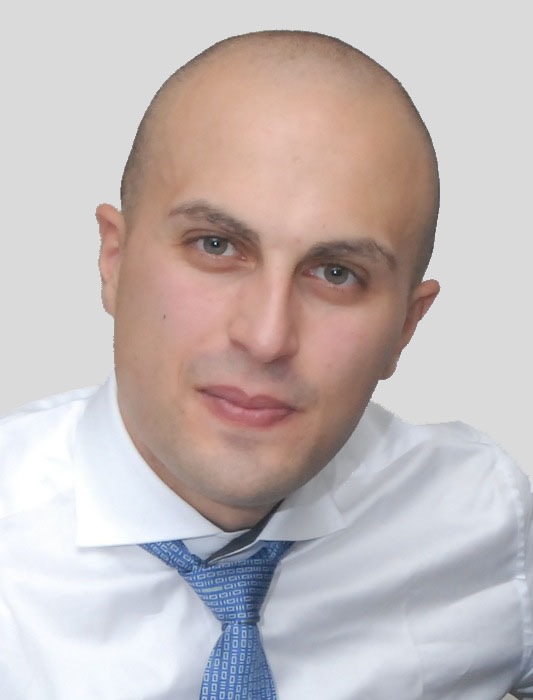
\includegraphics[width=1in,height=1.25in,clip,keepaspectratio]{pictures/cg}}]{Michael Shell}

%\end{IEEEbiography}

% if you will not have a photo at all:
\begin{IEEEbiographynophoto}{John Doe}
Biography text here.
\end{IEEEbiographynophoto}

% insert where needed to balance the two columns on the last page with
% biographies
%\newpage

\begin{IEEEbiographynophoto}{Jane Doe}
Biography text here.
\end{IEEEbiographynophoto}

% You can push biographies down or up by placing
% a \vfill before or after them. The appropriate
% use of \vfill depends on what kind of text is
% on the last page and whether or not the columns
% are being equalized.

%\vfill

% Can be used to pull up biographies so that the bottom of the last one
% is flush with the other column.
%\enlargethispage{-5in}



% that's all folks
\end{document}



